\appendix

\section*{Appendix}

%%%%%%%%%%%%%%%%%%%%%%%%%%%%%%%%%%%%%%%%%%%%%%%%%%%

\titlecontents{section}[18pt]{\vspace{0.05em}}{\contentslabel{1.5em}}{}
{\titlerule*[0.5pc]{.}\contentspage} % Set the formatting for appendix sections in the table of contents

\titlecontents{table}[0pt]{\vspace{0.05em}}{\contentslabel{1em}}{}
{\titlerule*[0.5pc]{.}\contentspage} % Set the formatting for appendix tables in the list of tables

\startcontents[appendix] % Start the table of contents for the appendix
\section*{Table of Contents} % Title for the appendix table of contents
%\addcontentsline{toc}{section}{Table of Contents} % Add the appendix table of contents to the main table of contents
\printcontents[appendix]{section}{0}{\setcounter{tocdepth}{4}} % Print the table of contents for the appendix

\startlist[appendix]{lot} % Start the list of tables for the appendix
\section*{List of Tables} % Title for the appendix list of tables
%\addcontentsline{lot}{section}{List of Tables} % Add the appendix list of tables to the main list of tables
\printlist[appendix]{lot}{}{\setcounter{tocdepth}{1}} % Print the list of tables for the appendix


\startlist[appendix]{lof} % Start the list of tables for the appendix
\section*{List of Figures} % Title for the appendix list of tables
%\addcontentsline{lot}{section}{List of Tables} % Add the appendix list of tables to the main list of tables
\printlist[appendix]{lof}{}{\setcounter{tocdepth}{1}} % Print the list of tables for the appendix


\newpage
%%%%%%%%%%%%%%%%%%%%%%%%%%%%%%%%%%%%%%%%%%%%%%%%%%%

\section{Related Work} \label{app:related-work}

Identifying the legal statutes and relevant prior cases given a legal fact or situation is one of the most fundamental tasks in law.
Traditionally, researchers have used statistical and lexical approaches to solve both tasks independently. The advent of deep learning NLP approaches has led to renewed efforts in both tasks using advanced architectures.

\vspace{1mm}
\noindent\underline{\bf Overview of Prior Works:} \label{sec:relwork/overview}
Traditional approaches for identifying relevant statutes and precedents have mostly involved exploiting lexical features such as n-grams of words~\citep{salton1988termweight}, hand-crafted features~\citep{zeng2007knowledge} or embeddings from pre-trained models like Doc2vec~\citep{le2014doc2vec}.
Lately, transformer-based embedding methods have been used for directly calculating dot product scores between the query and statute/precedent~\citep{vold2021tflegal}.
While most unsupervised approaches have utilized methods like Vector Space Model~\citep{salton1975vector} and BM25~\citep{robertson2009bm25}, supervised approaches for both tasks can broadly be divided into classification~\citep{liu2023ml,hofmann2013balancing} (model predicts similarity between query and statute/precedent) and ranking based~\citep{wang2018modeling,ma2022incorporating} (model ranks a list of statutes/precedents based on relevance to the query) approaches. 

\vspace{1mm}
\noindent\underline{\bf Identifying Legal Statutes:} \label{sec:relwork/statutes}
Historically, researchers have used multi-label learning frameworks to identify relevant statutes for a query~\citep{wang2018modeling,wang2019hmn,chalkidis2019neural}. In many jurisdictions, identifying the relevant statutes is considered to be a subtask of the broader task of Legal Judgment Prediction~\citep{zhong2018topjudge}, which could entail predicting the legal charges and term of punishment as auxiliary tasks.
Some approaches have only considered the text of the queries in the classification pipeline, relying on the encoder to generate good quality representations of the query~\citep{chalkidis2019neural}.
Others have incorporated the text of the statutes as well, in generating statute-aware query representations which are then used for classification~\citep{wang2018modeling,wang2019hmn}.
It should be noted that most of these approaches have worked in a setup with limited number of statutes (< 200), and hence the classification approach suffices.
Lately, LLMs have been used to perform the task of statute identification~\citep{wu2023precedent}, and these models can utilize their superior language understanding capabilities as well as knowledge of legal statutes to perform relatively better in the task of statute identification.

\vspace{1mm}
\noindent\underline{\bf Identifying Prior Cases:} \label{sec:relwork/precedents}
Unlike statutes, most prior works on prior case retrieval have modeled the task in a ranking framework. The major challenge in this task is the fact that both the queries and precedents are very long. 
Additionally, it has been observed that the query consists of several legal aspects, and each individual aspect leads to matching with certain precedents that eventually get cited~\citep{rabelo2022semantic}. 
Mostly, researchers have tried to reduce the noise in the query text by using event information~\citep{joshi2023ucreat,tang2024casegnn}, or extracting salient portions of the document~\citep{qin2024ljpretrieval}. 
\citet{rabelo2022semantic} took a granular approach, by dividing both the queries and precedents into paragraphs/sentences, scoring each pair of query and precedent sentence, and then generating aggregate scores.
Other approaches have involved usage of GNNs~\citep{tang2024casegnn,tang2024caselink}, citation network structures~\citep{bhattacharya2020hierspcnet}, making use of the statutes cited from the precedent cases (not the queries)~\citep{qin2024ljpretrieval}, and re-ranking approaches based on some first stage retriever like BM25~\citep{ma2021retrieving}.
LLMs have also been lately used to summarize the queries and precedents~\citep{qin2024ljpretrieval}, or perform query expansion based on its inherent domain knowledge~\citep{ma2024llmrelevance}.

%%%%%%%%%%%%%%%%%%%%%%%%%%%%%%%%%%%%%%%%%%%%%%%%%%
% \section{Dataset Construction Details}
% \label{sec:dataset-appendix}

% This section describes the procedure of constructing the IL-PCSR dataset in details. 
% As described briefly in \S~\ref{sec:dataset/overview}, we collected 20k case judgment documents from \url{indiankanoon.org}.

% \noindent We first perform simple pre-processing of the collected documents, such as removal of consecutive punctuations, whitespace, etc., spelling correction, and filtering gibberish text patterns. These errors are seen in legal case documents since in many cases the digital versions of the cases available on IndianKanoon might have been generated using automated OCR methods.

% \noindent To designate our query set and statute and precedent candidate pools, we next follow the steps described below. Also, to note, in our setting, training, validation and testing all share the same candidate pool.

% \noindent (i)~\textbf{Filtering by length:} We measured the length (in terms of number of tokens after NLTK~\citep{loper2002nltk} tokenization) of all the documents in our corpus, and removed very small ($<5$ percentile, approx. 400 tokens) and very large ($>95$ percentile, approx. 10k tokens) cases, giving us approx 18k cases.

% \noindent (ii)~\textbf{Intermediate Statute Pool:} We collected all the statutes (Sections/Articles from Central Govt. Acts) cited across all the 18k cases. We only choose those statutes that are cited at least 5 times across 18k cases, giving us an intermediate statute set of around 1200 statutes. However, we still add some statues having frequency < 5, to conform to a real-world setting where many non-relevant candidates may be present in the pool.

% \noindent (iii)~\textbf{Intermediate Precedent Pool:} We also enumerated all the prior cases cited from these 18k cases, which are also part of our corpus. We only choose those precedents that are cited at least 3 times across 18k cases, giving us an intermediate precedent set of around 5k documents. Similar to statutes, we also some add precedent cases that are cited less than 3 times.

% \noindent (iv)~\textbf{Final Query Set:} From our pool of 18k cases, we choose those cases that cite at least one statute and two precedents from their respective intermediate pools. This gives us a final query set of 6271 queries. This set was randomly divided into train/dev/test splits in the ratio of 80\%:10\%:10\%, giving us train, dev and test sets of sizes 5021, 627 and 627 respectively.

% \noindent (v)~\textbf{Final Statute and Precedent Pools:} Finally, we filter our intermediate candidate pools further, since we want those candidates that are cited more across the final query set. However, we also want to retain a few candidates in the test set that are unseen in train and dev sets (held-out candidates), to conform to a real-world setting.
% We sample few statutes that are cited less to satisfy the above property. 
% This process gives us a final statute pool of 936 statutes. We apply a similar policy for precedents, giving us a final precedent pool of 3183 cases.
% Of the 936 statutes, 19 are not cited from any query, and 29 are cited only from the test set but not the train set (held-out). Similarly, of the 3183 precedents, 94 are not cited from any query and 157 are held-out candidates.
% % More details can be found in Table~\ref{tab:dataset_stats}.

% \noindent (vi)~\textbf{Anonymization and Masking Citations:} We mask the portions of the query document where the citation occurs, to prevent deep learning models from associating the queries with the Section numbers, Act names or Case titles. Apart from these, we also anonymize the documents with regard to person names to prevent ethnic/religious biases. We utilize the LegalNER~\citep{kalamkar2022legalner} tool by Opennyai, which is capable of extracting mentions of Section numbers, Act names, Case titles, as well as entity names, to fair degree of accuracy. We replace the actual text with placeholders such as [SECTION], [ACT], [PRECEDENT] and [ENTITY]. 

\section{Dataset Construction Details}
\label{sec:dataset-appendix}

This section details the construction pipeline for the \ilpcsr\ dataset. As noted in \S~\ref{sec:dataset/overview}, we collected 20k case judgment documents from \url{indiankanoon.org}, a widely used legal search engine in India.  

\vspace{1mm}
\noindent\underline{\textbf{Pre-processing:}} The raw documents were normalized through standard text-cleaning operations, including removal of redundant punctuation and whitespace, spelling correction, and filtering of malformed strings. Such artifacts are common in legal case records, as many judgments on IndianKanoon originate from scanned archives processed via OCR, which often introduces typographical noise.  

\vspace{1mm}
\noindent\underline{\textbf{Query and Candidate Pool Construction:}} We then derived the query set and candidate pools of statutes and precedents through the following steps. Detailed statistics are reported in Table~\ref{tab:salient-stats-ilpcsr}. Note that in our setup, training, validation, and test sets all share the same candidate pool.  

% \begin{enumerate}[label=(\roman*)]
\noindent (i)~\textbf{Filtering by length:} We measured document length in tokens using NLTK~\citep{loper2002nltk} tokenization. Extremely short ($<$5th percentile, $\sim$400 tokens) and extremely long ($>$95th percentile, $\sim$10k tokens) cases were removed, yielding a working corpus of $\sim$18k judgments.  

\noindent (ii)~\textbf{Intermediate statute pool:} From these 18k cases, we extracted all statutes (sections/articles from Central Government Acts) cited. To suppress spurious candidates, we retained only statutes cited at least five times, producing an intermediate pool of $\sim$1200 statutes. A small number of low-frequency statutes were also included to preserve the long-tail distribution typical of real-world scenarios.  

\noindent (iii)~\textbf{Intermediate precedent pool:} Likewise, we enumerated all cited prior cases in the 18k corpus. Precedents cited at least three times were retained, giving an intermediate pool of $\sim$5k documents. As with statutes, a subset of infrequent precedents was deliberately retained for distributional realism.  

\noindent (iv)~\textbf{Final query set:} We then selected cases citing at least one statute and at least two precedents from the intermediate pools, resulting in 6,271 queries. These were partitioned into training, development, and test splits in an 8:1:1 ratio (5,021 / 627 / 627).  

\noindent (vi)~\textbf{Final candidate pools:} The intermediate statute and precedent pools were refined to better reflect frequency distributions in the final query set, while retaining a subset of rare candidates to act as held-out items in evaluation. The final statute pool contains 936 statutes (19 never cited, 20 held-out) and the final precedent pool contains 3,183 cases (93 never cited, 88 held-out). Refer to Table~\ref{tab:salient-stats-ilpcsr} for a snapshot of the salient statistics. 

\vspace{1mm}
\noindent \underline{\textbf{Anonymization and masking:}} To prevent models from directly exploiting citation strings, we masked all portions of query texts where explicit references occurred (section numbers, Act names, or case titles). Additionally, to mitigate potential bias, all personal names were anonymized using the LegalNER tool~\citep{kalamkar2022legalner}, which identifies statutory references, case titles, and entity mentions with high reliability. Identified spans were replaced with standardized placeholders: [SECTION], [ACT], [PRECEDENT] and [ENTITY].  
% \end{enumerate}

\vspace{1mm}
\noindent\underline{\bf Distribution of Categories:}
Based on discussions with legal experts, all queries, precedents, and statutes were categorized into 13 broad legal domains (Table~\ref{tab:categories}). The distribution is highly skewed: categories such as \textit{Criminal} and \textit{Property \& Land Disputes} dominate, whereas others like \textit{IPR} and \textit{Environmental} are sparsely represented. This skew reflects the real-world case distribution observed in Indian courts.

% Requires: \usepackage{graphicx}
\begin{table}[h]
    \centering
    \small
    \begin{tabular}{lccc}
        \hline
        \textbf{Category} & \textbf{Stats} & \textbf{Precs} & \textbf{Queries} \\
        \hline
        Labour \& Employment & 36  & 219 & 316  \\
        Criminal & 316 & 959 & 2240 \\
        Income Tax & 134 & 363 & 683 \\
        Motor Vehicle Accidents & 27  & 176 & 413  \\
        Family \& Marriage & 24  & 59  & 236  \\
        Property \& Land Disputes & 91  & 403 & 950  \\
        Contract \& Commercial & 77  & 193 & 400  \\
        Constitutional & 153 & 463 & 283  \\
        Intellectual Property Rights & 9   & 29  & 20   \\
        Consumer Protection & 10  & 23  & 46   \\
        Environmental & 9   & 23  & 10   \\
        Company \& Corporate & 40  & 16  & 83   \\
        Service Matters & 10  & 249 & 586  \\
        \hline
    \end{tabular}
    \caption{Distribution of Statutes, Precedents, and Queries across various categories}
    \label{tab:categories}
\end{table}


%%%%%%%%%%%%%%%%%%%%%%%%%%%%%%%%%%%%%%%%%%%%%%%%%%
%%%%%%%%%%%%%%%%%%%%%%%%%%%%%%%%%%%%%%%%%%%%%%%%%%%


% \section{Details of Implementation \& Experimental Setup} \label{app:implementation}

% \noindent\textbf{Setup and Hyperparameters:} For BM25-based experiments, we used different n-grams ($n=2,3,4,5$). In case of the fine-tuning approaches, we use a contrastive learning setup, with BM25 hard negatives and in-batch negative sampling. We used  AdamW~\citep{loshchilov2017adamw} optimizer and a linear scheduler. For re-ranking, we used GPT-4.1 and chose top $k=20$ for statutes and $k=10$ for precedents.

% All GPU-based experiments were conducted on a single Nvidia RTX A100 80 GB GPU. The details of individual models are as follows. The compute costs and time for different experiments are listed in Table~\ref{tab:computecosts}.

% \noindent\textbf{BM25:} For BM25 experiments, both in default settings as well as event-filtered sentences (SpaCy or LLM), we experimented with n-gram=2. The vocabulary construction was performed with $\textrm{min\_df}=1$ document and $\textrm{max\_df}=65\%$ of the corpus. We also set $b=0.7$ and $k_1=1.6$.

% \noindent\textbf{SpaCy Events:} For event extraction, we used the \texttt{en-core-web-trf} model for SpaCy and followed the same steps as \citet{joshi2023ucreat}. 

% \noindent\textbf{LLM Events:} As described in Section~\ref{sec:method}, we used the SALI ontology to obtain definitions of events to be provided to LLMs. We chose 18 top-level nodes as entity types, and asked the LLM to extract meaningful verbs/phrases signifying the action or relation between the head and tail entities.  Specifically, the exact prompt is described in Table~\ref{tab:event-llm-prompt}. Figure~\ref{fig:eventgnn} shows a sub-graph of the events generated for a sample document.
% We first used \texttt{GPT-4-turbo} to obtain the events for a small set of documents ($\sim 400$). Thereon, we used a smaller, open model \texttt{gemma-7b-it} and fine-tuned over the GPT outputs, to be able to mimic the performance of GPT for event extraction. This fine-tuned Gemma model was subsequently used to obtain the events for the entire dataset (queries and precedents). We followed this pipeline to replicate the superior performance of GPT at lesser financial expense.

% \noindent\textit{Hyper-parameters for Gemma:} For fine-tuning the Gemma model, we used a batch size of 4, l.r. 2e-4 and trained the model for 10 epochs using PEFT. We used 4-bit quantization and $r=8, \alpha=16$ for LoRA parameters. During inference, we used a batch size of 1 and greedy search decoding.

\begin{table*}
    \centering
    \begin{tabular}{|p{0.99\textwidth}|}
    \hline
        As an Indian lawyer, your job is to understand legal documents. Right now, you're building a detailed knowledge graph based on information in a given legal document. 
It's crucial that this graph includes all the fact, evidences, observations  from the document, so nothing important is left out.
The goal is to make legal analysis easier by focusing on the key information and skipping the obvious stuff.
        \\
        Each triplet should be in the form of (h:type, r, o:type), where 'h' stands for the head entity,
'r' for the relationship, and 'o' for the tail entity. The 'type' denotes the category of the corresponding entity.
        \\
        The Entities should be non-generic and can be classified into the following categories:
        \\
        - Actor / Player: A person who has a role in a legal matter (e.g., Buyer, Provider, Lawyer, Law Firm, Expert, Employer, Employee, Buyer, Seller, Lessor, Lessee, Debtor, Creditor, Payor, Payee, Landlord, Tenant).
\\
- Area of Law: The practice area into which a legal matter or legal area of study falls (e.g., Criminal Law, Real Property Law, Mergers and Acquisitions Law, Personal and Family Law, Tax and Revenue Law).
\\
- Asset Type: Type of resource that is owned or controlled by a person, business, or economic entity
\\
- Communication Modality: Entities' chosen communication method (e.g., written, email, telephone, portal), as well as time (e.g., synchronous, asynchronous).
\\
- Currency: A standardization of money that is used, circulated, or exchanged (e.g., banknotes, coins).
\\
- Document / Artifact: A written, drawn, presented, or memorialized representation of thought or expression, including evidence such as recordings and other artifacts.
\\
- Engagement Terms: Terms to define an engagement for providing legal services.
\\
- Event: A matter's events, as well as collections of those events (often noted as "phases").
\\
- Forums and Venues: Organization or government entity that administers proceedings.
\\
- Governmental Body: Administrative entities of government or state agency or appointed commission, as a permanent or semi-permanent governmental organization that oversees or administers specific governmental functions.
\\
- Industry: An economic branch that produces a related set of raw materials, goods, or services (e.g., Agriculture Industry, Pharmaceuticals Industry).
\\
- Legal Authorities: Documents or publications that guide legal rights and obligations (e.g., caselaw, statutes, regulations, rules) or that can be cited as providing guidance on the law (e.g., secondary legal authorities).
\\
- Legal Entity: A person, company, organization, or other entity that has legal rights and obligations.
\\
- Location: The name of a position on the Earth, usually in the context of continents, countries, and their political subdivisions (e.g., regions, states or provinces, cities, towns, villages).
\\
- Matter Narrative: A textual narrative of a matter's factual and legal details.
\\
- Objectives: Specific aims, goals, arguments, plans, intentions, designs, purposes, schemes, etc. that are constructed by a party in a legal matter, and the legal or other professional frameworks that support their execution.
\\
- Service: The legal work performed, usually by a Legal Services Provider, in the course of a legal matter.
\\
- Status: The state or condition of a proceeding, legal element, or legal matter (e.g., open, closed, canceled, expired).
\\
The Relationships r between these entities must be represented by meaningful verbs/actions and its  properties  like cause purpose manner etc .
\\
Remember to conduct entity disambiguation, consolidating different phrases or acronyms that refer to the same entity.
Simplify each entity of the triplet to be no more than three or four words.
\\
Include triplets that are implicitly inferred from the document's context but not explicitly stated, in order to ensure the graph is both connected and dense. \\ \hline     
    \end{tabular}
    \caption{Prompt used for LLM events}
    \label{tab:event-llm-prompt}
\end{table*}

\section{Details of Implementation \& Experimental Setup} \label{app:implementation}

All experiments were conducted on a single Nvidia RTX A100 80 GB GPU. Unless otherwise noted, all training runs used mixed precision (fp16) and fixed random seed (42).  

\noindent \textbf{BM25:} We implemented BM25 with n-grams ($n=2,3,4,5$). Vocabulary was constructed with $\texttt{min\_df}=1$ and $\texttt{max\_df}=65\%$, and BM25 hyperparameters were fixed at $b=0.7$ and $k_1=1.6$. BM25 was run in two variants: full-document input and event-filtered input (SpaCy or LLM).  

\noindent \textbf{Event generation:} We used two pipelines. The SpaCy-based pipeline used the \texttt{en-core-web-trf} model following \citet{joshi2023ucreat}. The LLM-based pipeline leveraged the SALI ontology with 18 top-level entity types, prompting the LLM to extract verbs/phrases as relations between entities. To control costs, we first used \texttt{GPT-4-turbo} to annotate $\sim$400 documents, then fine-tuned \texttt{gemma-7b-it} on this output. The fine-tuned Gemma model was subsequently used to process the entire dataset, providing GPT-level quality at lower expense.  

\noindent \textbf{SAILER:} We used the fine-tuned English checkpoint \texttt{CSHaitao/sailer-en-finetune}. Paragraphs were truncated at 512 tokens and encoded using CLS pooling without normalization. Similarity was computed via dot product.  

\noindent \textbf{Ensemble Methods:} In the ensemble setup (Figure~\ref{fig:ensemble}), lexical and semantic scores are combined using the weighting parameter $\alpha$. $\alpha$ was either tuned via grid search in $[0,1]$, or dynamically estimated from query embeddings using a feed-forward network with sigmoid activation.  

\noindent \textbf{LLM Re-ranking:} For LLM re-ranking, we used GPT-4.1, selecting top-$k=20$ statutes and top-$k=10$ precedents from first-stage retrieval for re-ranking. All LLM prompts were executed with deterministic decoding ($\texttt{temperature}=0$), without explicit max token or stop constraints.  

\begin{table*}
    \centering
    \begin{tabular}{|p{0.99\textwidth}|}
    \hline
    Summarize the key points from a provided case document that contributed to the final judgment. These summaries will later be used to identify the reasons why this case might be cited as a precedent. Please process the given legal precedent and focus on the following instructions:
\\
    Objective:  Identify and extract the key legal findings, principles, or rules established in this precedent that could serve as the basis for its citation in other judgments.
\\
    Structure: Each key points should be phrased in a concise and neutral manner.Avoid including case-specific details (e.g., names, dates, or specific statutes cited).
                             Ensure the summaries comprehensively capture the reasons, enabling effective matching with those from the queries.
\\
                    Focus Areas: Prioritize the sections where legal principles are established, clarified, or interpreted, 
                    focusing on the parts likely to be cited as precedents. \\ \hline
    \end{tabular}
    \caption{Prompt used for precedent summarization}
    \label{tab:prec-summ-prompt}
\end{table*}

\begin{table*}
    \centering
    \begin{tabular}{|p{0.99\textwidth}|}
    \hline
    Extract legal incidents from a given judgment to understand why specific sections or articles of law
                    were cited. These extracted incidents will later be matched with relevant sections and articles.
\\
                    Please process the given legal judgment and focus on the following instructions:
\\
                    Objective: Identify and extract all legal incidents referenced in the judgment, 
                    focusing on the key facts and legal issues of the case.
\\
                    Structure: Phrase each incident concisely and neutrally.
                    Exclude case-specific details (e.g., names, dates, case numbers).
                    The extracted incidents should be rich in legal reasoning and sufficiently descriptive to enable accurate section/article matching.
\\
                    Focus Areas: Capture the core facts and issues underlying the case. \\ \hline
    \end{tabular}
    \caption{Prompt used for query summarization w.r.t. LSR}
    \label{tab:qry-summ-prompt-statwise}
\end{table*}

\begin{table*}
    \centering
    \begin{tabular}{|p{0.99\textwidth}|}
    \hline
    Extract reasons from a legal judgment (query) explaining why the judge cited specific precedents
                    , to later match these reasons with findings from the cited precedents for retrieval tasks.
                    Please process the given legal judgment and focus on the following instructions:
\\
                    Objective: Identify and extract all the legal reasons cited in the given judgment, 
                    focusing on the legal principles, rules, or questions of law discussed or evaluated. 
                    Exclude any specific factual context or case-specific details.
\\
                    Structure: Each reason should be phrased in a concise and neutral manner.
                            Avoid including case-specific details (e.g., names, dates, or specific statutes cited).
                            Ensure the reasons are comprehensive enough to match with similar principles from other precedents.
\\
                    Focus Areas: While extracting reasons, focus only the places where the precedents and cited text is present. \\ \hline
    \end{tabular}
    \caption{Prompt used for query summarization w.r.t. PCR}
    \label{tab:qry-summ-prompt-precwise}
\end{table*}

\subsection{Fine-tuning Setup} \label{sec:expt/implementation/ft}

All fine-tuning experiments used a cross-entropy loss in a contrastive learning setup. Each query was paired with one positive candidate and BM25 hard negatives. In-batch negatives were also used, ensuring each positive candidate appeared at least once during training. %For multi-task experiments, losses were combined with a 3:7 weighting between statute and precedent retrieval.  
Training was performed with AdamW optimizer ($\texttt{weight\_decay}=1\mathrm{e}{-2}$), linear decay schedule with warmup (10\% of total steps), and evaluation at the end of each epoch. Early stopping was not used; instead, all checkpoints were evaluated and the best dev F1 was selected.  

\noindent\textbf{Gemma (event generation):} Batch size 4, learning rate $2\times10^{-4}$, 10 epochs, trained with PEFT using 4-bit quantization via \texttt{bitsandbytes}. LoRA parameters: $r=8$, $\alpha=16$. Inference used batch size 1 and greedy decoding.  

\noindent\textbf{SAILER:} Batch size 4, one positive and three negatives per query, 20 epochs, peak learning rate $5\times10^{-6}$.  

\noindent\textbf{GNN-based methods:} Both Event-GNN and Para-GNN used two-layer Graph Attention Networks with dropout of $0.1$, Node and edge embeddings were initialized with SentenceBERT~\citep{reimers2019sentencebert}. Training used batch size 32, one positive and 999 negatives per query, 100 epochs, peak learning rate $1\times10^{-4}$.  



\subsection{Prompts for LLMs} \label{app:prompts}
We utilized different LLMs at three distinct stages of experiments. We used a teacher-student LLM setup (using GPT-4 and Gemma) for generating events, and GPT-4o-mini for generating summaries. Here, the LLMs are used as a pre-processor. Apart from these, we use GPT-4.1 for the direct retrieval task using a re-ranking framework.

\vspace{1mm}
\noindent \underline{\bf Event generation:} We used the SALI ontology with 18 top-level entity types, prompting the LLM to extract verbs/phrases as relations between entities. Some of these entities include `actor', `asset type', `legal authorities' and so on (full details in Table~\ref{tab:event-llm-prompt}).

\vspace{1mm}
\noindent \underline{\bf Summary generation:} To reduce noise and computational cost, we used \texttt{GPT-4o-mini} for retrieval-oriented summarization, as discussed in \S~\ref{sec:method}.  
For \textbf{precedents}, prompts targeted the \textit{legal findings and rulings} that justify their citation (Table~\ref{tab:prec-summ-prompt}).  
For \textbf{queries}, two separate prompts were used: (i) an LSR-oriented prompt focusing on \textit{facts and legal issues} (Table~\ref{tab:qry-summ-prompt-statwise}); and (ii) a PCR-oriented prompt focusing on \textit{arguments, reasoning, and lower court findings} (Table~\ref{tab:qry-summ-prompt-precwise}). This dual setup reflects that statute and precedent retrieval rely on different contextual signals.  

\vspace{1mm}
\noindent \underline{\bf LLM Re-ranking:} For LLM-based re-ranking (see \S~\ref{sec:method}), prompts differed by task:  
For LSR, a single prompt (Table~\ref{tab:qry-stat-rerank}) was used for both stages, with Stage 2 extending the candidate pool using statutes cited by Stage 1 precedents.  
PCR involved two separate prompts. Stage 1 (Table~\ref{tab:qry-prec-rerank1}) asked the LLM to predict whether a masked query cites a given precedent. Stage 2 (Table~\ref{tab:qry-prec-rerank2}) added statute information from both query and precedent, allowing the LLM to exploit cross-task dependencies.  







% \noindent\textbf{SAILER:} For SAILER, we used the fine-tuned English model available at \texttt{CSHaitao/sailer-en-finetune}. We encoded each paragraph using the model (first 512 tokens), and then took the average embedding as the final representation. We then calculated dot product over these embeddings.

% \noindent\textbf{Ensemble Model:} The workflow of the Ensemble-based models is shown in Figure~\ref{fig:ensemble}. The parameter $\alpha$ can either be derived using grid search over a range of values $\in [0, 1]$, or learnt from the semantic embedding of the query using a feed-forward network (FFN) with sigmoid activation.



% \subsection{Fine-tuning Setup} \label{sec:expt/implementation/ft}

% For fine-tuning experiments, we used a contrastive learning setup. To elaborate, for every query, we sampled a single positive candidate and a fixed number of BM25 hard negative candidates.
% We also used in-batch sampling, where in, positives for other queries in a batch can be considered as negatives for the current query. 
% We also ensured each positive candidate for each query was seen during training.
% For the multi-task experiments, we took a ratio of 3:7 for statute to precedent loss.

% \noindent\textbf{SAILER:} For SAILER fine-tuning, we used a batch size of 4, 1 positive and 3 negative examples per query, and trained the model for 20 epochs with a  peak l.r. of 5e-6.

% \noindent\textbf{GNN-based methods:} For both GNN-based methods, we use a 2-layer Graph Attention Network. All node and edge embeddings are initialized with SentenceBERT~\citep{reimers2019sentencebert}. We used a batch size of 32, 1 positive and 999 negative examples per query, and trained the model for 100 epochs with a peak l.r. of 1e-4. 


% \subsection{Setup and Prompts for Summarization} \label{sec:expt/implementation/summ}

% As described in Section~\ref{sec:method}, we used an LLM \texttt{(GPT-4o-mini)} to summarize both the precedents (candidate cases) and queries to reduce noise and ease computation overhead during both training and inference. We asked the LLM to perform a retrieval-focused summarization, focusing on the reasons for citation. 

% For precedents, we asked the model to focus on the legal findings and rulings of the court (prompt given in Table~\ref{tab:prec-summ-prompt}). 
% For queries, we used two separate prompts to focus on the legal facts and issues (for statutes -- see Table~\ref{tab:qry-summ-prompt-statwise}) and arguments and lower court findings (for precedents -- see Table~\ref{tab:qry-summ-prompt-precwise}).




% \subsection{LLM Re-ranking Prompts} \label{app:expt/llm}

% The prompt used for LLM re-ranking of statutes is displayed in Table~\ref{tab:qry-stat-rerank}. The same prompt is used in both stages, since for the second stage we just have a larger pool to re-rank from. However, in the case of PCR, Table~\ref{tab:qry-prec-rerank1} shows the first-stage prompt, and Table~\ref{tab:qry-prec-rerank2} shows the second-stage prompt, which additionally includes the statute information.     

\subsection{Evaluation Metrics} \label{app:expt/datasets}

We use macro-F1@$k$ scores for evaluation. We follow the same evaluation scheme as followed by \citet{joshi2023ucreat}, wherein the scores for a particular method are calculated for all $k \in \{1, 2, \ldots, 10\}$ for the validation set, and the best $k$ is chosen for evaluation on the test set for that particular method. Apart from F1, we also report the Mean Average Precision (MAP) and Mean Reciprocal Rank (MRR) scores for all models.
We also perform statistical significance testing with the paired T-test over the best performing results (see Table~\ref{tab:sigtest}).

\begin{table}
    \centering
    \small
    \setlength{\tabcolsep}{5pt}
    \begin{tabular}{lcc}
    \toprule
        \textbf{Experiment} & \textbf{Cost} & \textbf{Time} \\
        \midrule
        \multicolumn{3}{c}{\textbf{Prediction Tasks}}\\ \midrule
        
        SAILER (inference) & 20 GB & 5m \\
        SAILER (fine-tuning) & 80 GB & 4h \\
        SAILER (summary inference) & 20 GB & 2m \\
        SAILER (summary fine-tuning) & 80 GB & 2h 30m \\
        Event-GNN & 30 GB & 35m \\
        Para-GNN (full doc)& 64 GB & 1h 20m \\
        Para-GNN (summary) & 45 GB & 45m\\
 Event-GNN + BM25, dyn. $\alpha$& 35 GB&40m\\
 Para-GNN (full doc) + BM25, dyn. $\alpha$& 80 GB&1h 30m\\
 Para-GNN (summary) + BM25, dyn. $\alpha$ & 60 GB&50m\\ \midrule
        \multicolumn{3}{c}{\textbf{Event and Summary Generation}}\\ \midrule 
        GPT-4 (events) & 25 USD & 3h\\
        Gemma (fine-tuning) & 80 GB & 4h 30m \\
        Gemma (inference) & 40 GB & 12h \\
        GPT-4o-mini (summaries) & 30 USD& 30h\\ \midrule
 \multicolumn{3}{c}{\textbf{LLM Re-ranking}}\\ \midrule
 GPT-4.1 (LSR Stage 1)& 5 USD&20m\\
 GPT-4.1 (LSR Stage 2)& 5 USD&20m\\
 GPT-4.1 (PCR Stage 1)& 70 USD&4h\\
 GPT-4.1 (PCR Stage 2)& 70 USD&4h\\ \bottomrule
    \end{tabular}
    \caption{Compute costs and runtime of different models. Time represents the time taken for each epoch in the case of training experiments.}
    \label{tab:computecosts}
\end{table}

\subsection{Compute Costs}~\label{app:expt/costs}

Table~\ref{tab:computecosts} summarizes the compute requirements of all experiments. For free models, we report GPU memory (GB) and wall-clock time; for API calls, costs are reported in USD. Training costs are given per epoch, while inference is total runtime. This breakdown highlights the trade-offs across lexical baselines (minimal compute), GNN-based methods (moderate GPU use), and LLM-based pipelines (higher API cost but superior performance).  




%%%%%%%%%%%%%%%%%%%%%%%%%%%%%%%%%%%%%%%%%%%%%%%%%%%



\section{Details of Results and Analyses} \label{app:results}


% To further understand the weightage being placed to the lexical and semantic approaches when merging the scores, we vary $\alpha = \{0.0, 0.1, 0.2, \ldots, 0.9, 1.0\}$ and plot both statute and precedent scores in Figures~\ref{fig:ensemble-statalpha},~\ref{fig:ensemble-precalpha} respectively. For the semantic method, we used Event-GNN for statutes, whereas we used RR-GNN for precedents, since these were the best performing methods for LSR and PCR respectively (Table~\ref{tab:results}). In both cases, vanilla BM25 was used as the lexical method, and we calculated the metrics for different n-grams of BM25 ($n = 2,3,4,5$). Here, $\alpha = 0$ represents pure lexical score while $\alpha=1$ represents pure semantic score.

% Figures~\ref{fig:ensemble-statalpha},~\ref{fig:ensemble-precalpha} demonstrates that a hybrid approach indeed works the best, for both statutes and precedents respectively. This holds true all the semantic methods, Event-GNN and Para-GNN (both with full documents and summaries as input), and also different n-grams of BM25. In almost all scenarios, the best performance is achieved at high values of $\alpha$, with the peak performance being achieved as high as $\alpha = 0.9$ in most cases. This indicates that for the semantic models, the scores being assigned to each query, candidate pair have less variance across candidates that are actually relevant versus those that are not, whereas BM25 scores have much higher variance. We also observe significant gains at the optimal $\alpha$ (ensemble score) compared to $\alpha=0$ (pure lexical score) or $\alpha=1$ (pure semantic score), for almost all settings.
% The only exception is Figure~\ref{fig:ensemble/eventprec} (PCR on Event-GNN ensemble), possibly since the pure semantic PCR score by Event-GNN is very low (12.08\% F1). 

\subsection{Optimal $\alpha$ values for ensemble models} \label{app:optimal-alpha}
The $\alpha$ term is responsible for deciding the balance between lexical and semantic components for ensemble methods. While this can be decided in static fashion by performing a grid search over the dev set, it can also be optimized dynamically (different optimal $\alpha$ for each query) by fine-tuning an FFN over the query embeddings (see \S~\ref{sec:method}).

\vspace{1mm}
\noindent \underline{\bf Grid Search:} To better understand the weighting between lexical and semantic components in our ensemble models, we performed a grid search over $\alpha = \{0.0, 0.1, \ldots, 1.0\}$, where $\alpha=0$ corresponds to pure BM25 and $\alpha=1$ to pure semantic scoring. Figures~\ref{fig:ensemble-statalpha} and \ref{fig:ensemble-precalpha} show the results for LSR and PCR, respectively, across different semantic methods (Event-GNN, Para-GNN with full documents, and Para-GNN with summaries) and BM25 variants ($n=2,3,4,5$).
For \textbf{LSR}, we observe peak performance at high $\alpha$ values (typically $0.8$–$0.9$), confirming that statutes benefit primarily from \textit{semantic reasoning} provided by GNNs, with BM25 adding complementary lexical grounding. In contrast, \textbf{PCR} peaks at moderately high $\alpha$ values ($0.7$–$0.8$) and deteriorates sharply near $\alpha=1$, highlighting the greater role of \textit{lexical overlap} in precedent retrieval. Importantly, in both tasks, the best results are never achieved at the extremes—ensembles consistently outperform either component alone.

\begin{table}[!ht]
\centering
\small
\begin{tabular}{lcc}
\hline
\textbf{Method} & \textbf{LSR $\alpha$} & \textbf{PCR $\alpha$} \\
\hline
Independent fine-tuning & 0.84 & 0.16 \\
Multi-task fine-tuning   & 0.94 & 0.79 \\
Transfer learning        & 0.85 & 0.81 \\
\hline
\end{tabular}
\caption{Average $\alpha$ values learned by the dynamic weighting method for statutes (LSR) and precedents (PCR).}
\label{tab:dynalpha}
\end{table}

\begin{figure*}
\begin{subfigure}[t]{.32\textwidth}
  \centering
  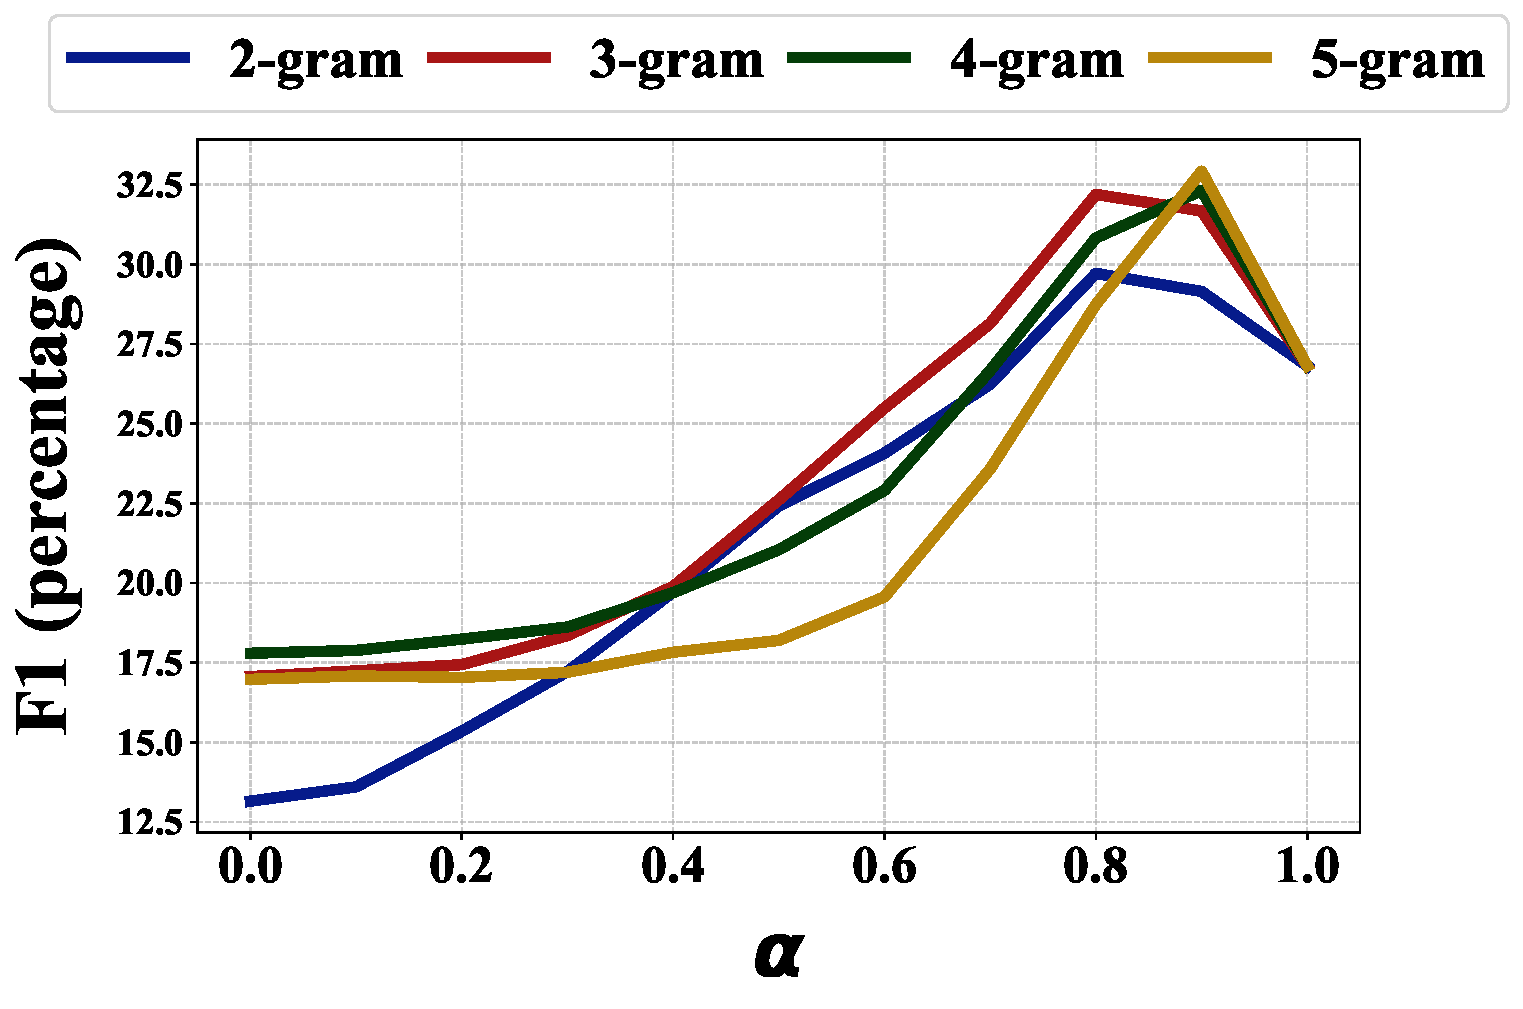
\includegraphics[width=\linewidth]{./images/ensemble-event-stat.pdf}
  \caption{LSR on Event-GNN + BM25}
  \label{fig:ensemble/eventstat}
\end{subfigure}%
\begin{subfigure}[t]{.32\textwidth}
  \centering
  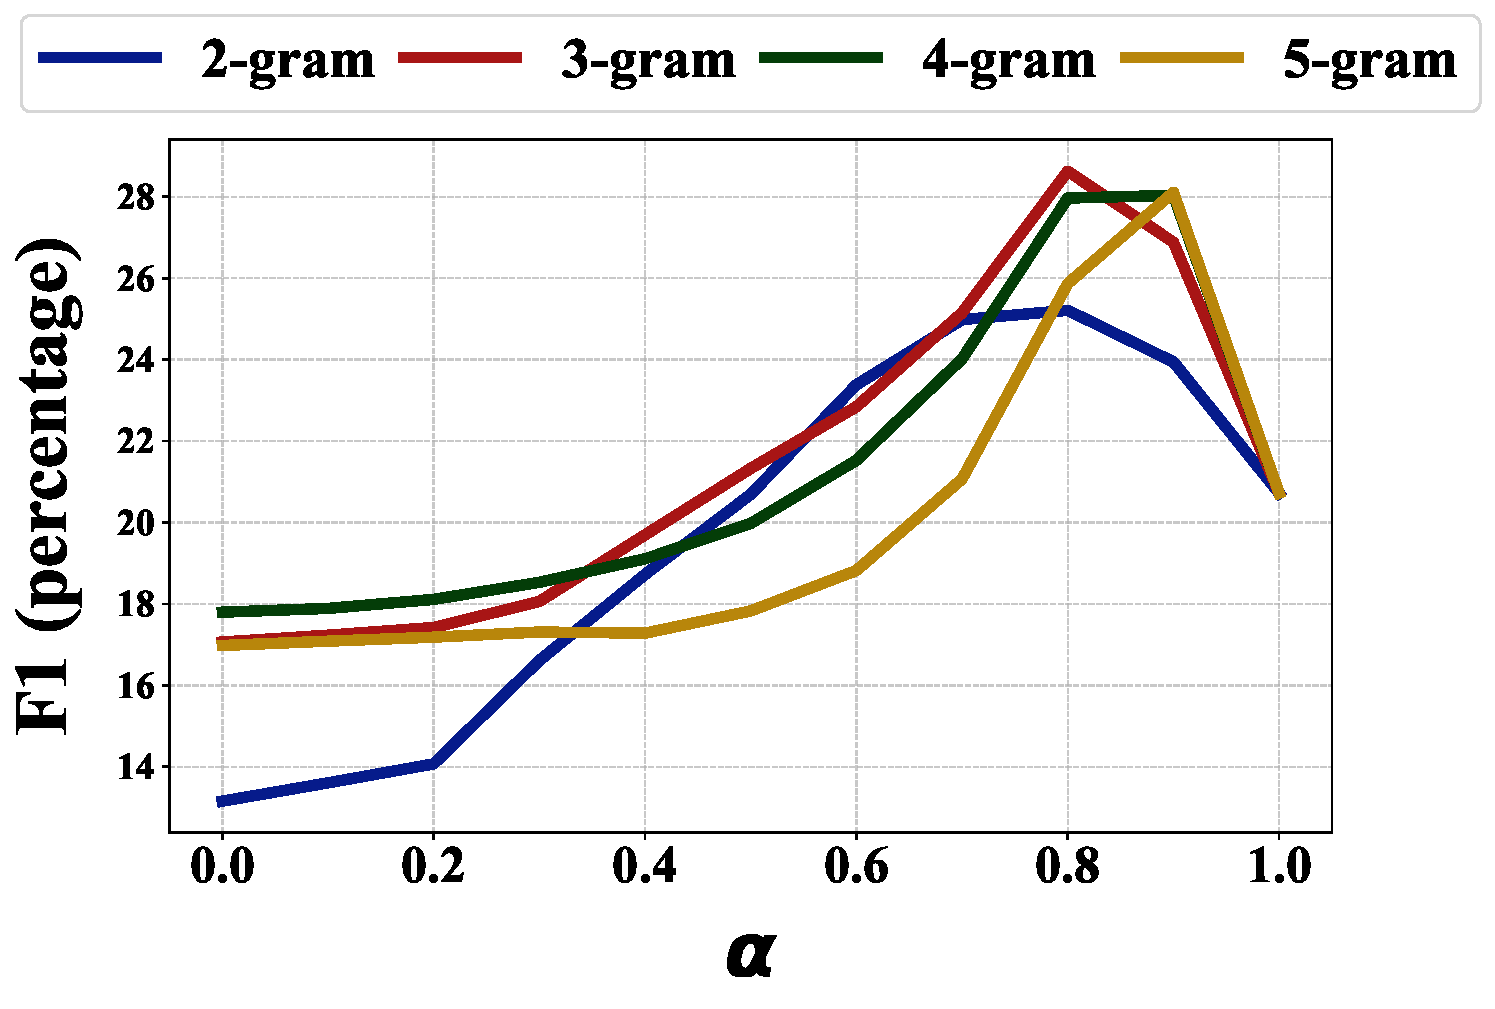
\includegraphics[width=\linewidth]{./images/ensemble-para-stat.pdf}
  \caption{LSR on Para-GNN + BM25}
  \label{fig:ensemble/parastat}
\end{subfigure}%
\begin{subfigure}[t]{.32\textwidth}
  \centering
  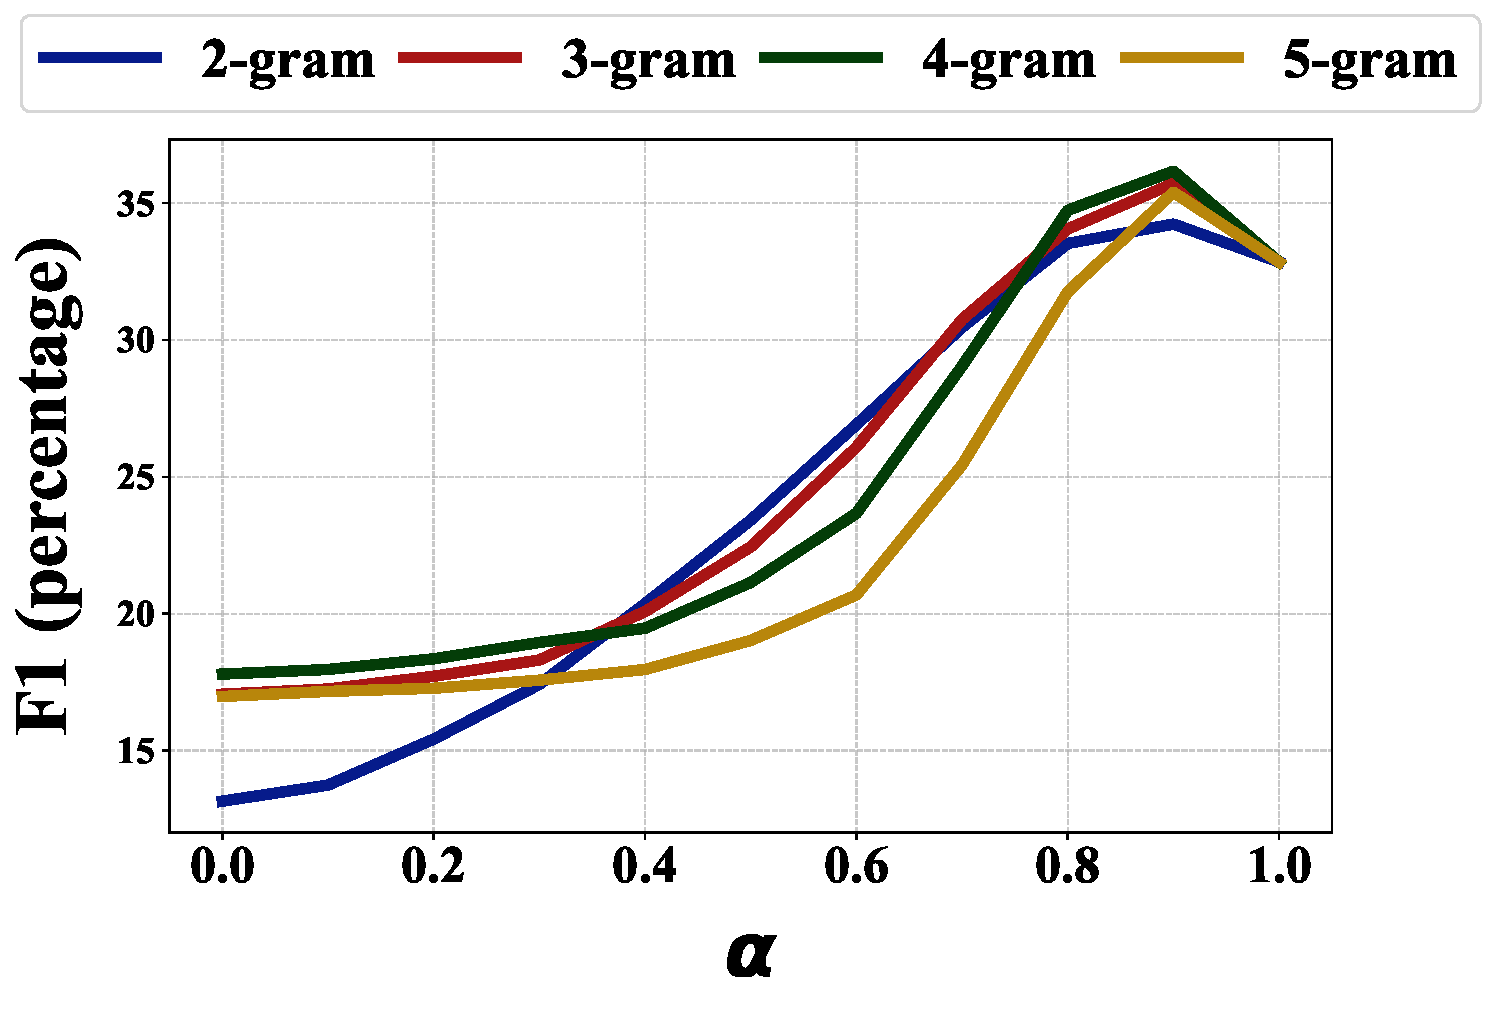
\includegraphics[width=\linewidth]{./images/ensemble-summ-stat.pdf}
  \caption{LSR on Para-GNN (summaries) + BM25}
  \label{fig:ensemble/summstat}
\end{subfigure}%
%\vspace{-4mm}
\caption{Grid Search F1(\%) of the ensemble methods for LSR task. Each figure shows the plot of performance vs. different $\alpha$ values when combining different models with BM25.} 
\label{fig:ensemble-statalpha}
%\vspace{-5mm}
\end{figure*}

\begin{figure*}
\begin{subfigure}[t]{.32\textwidth}
  \centering
  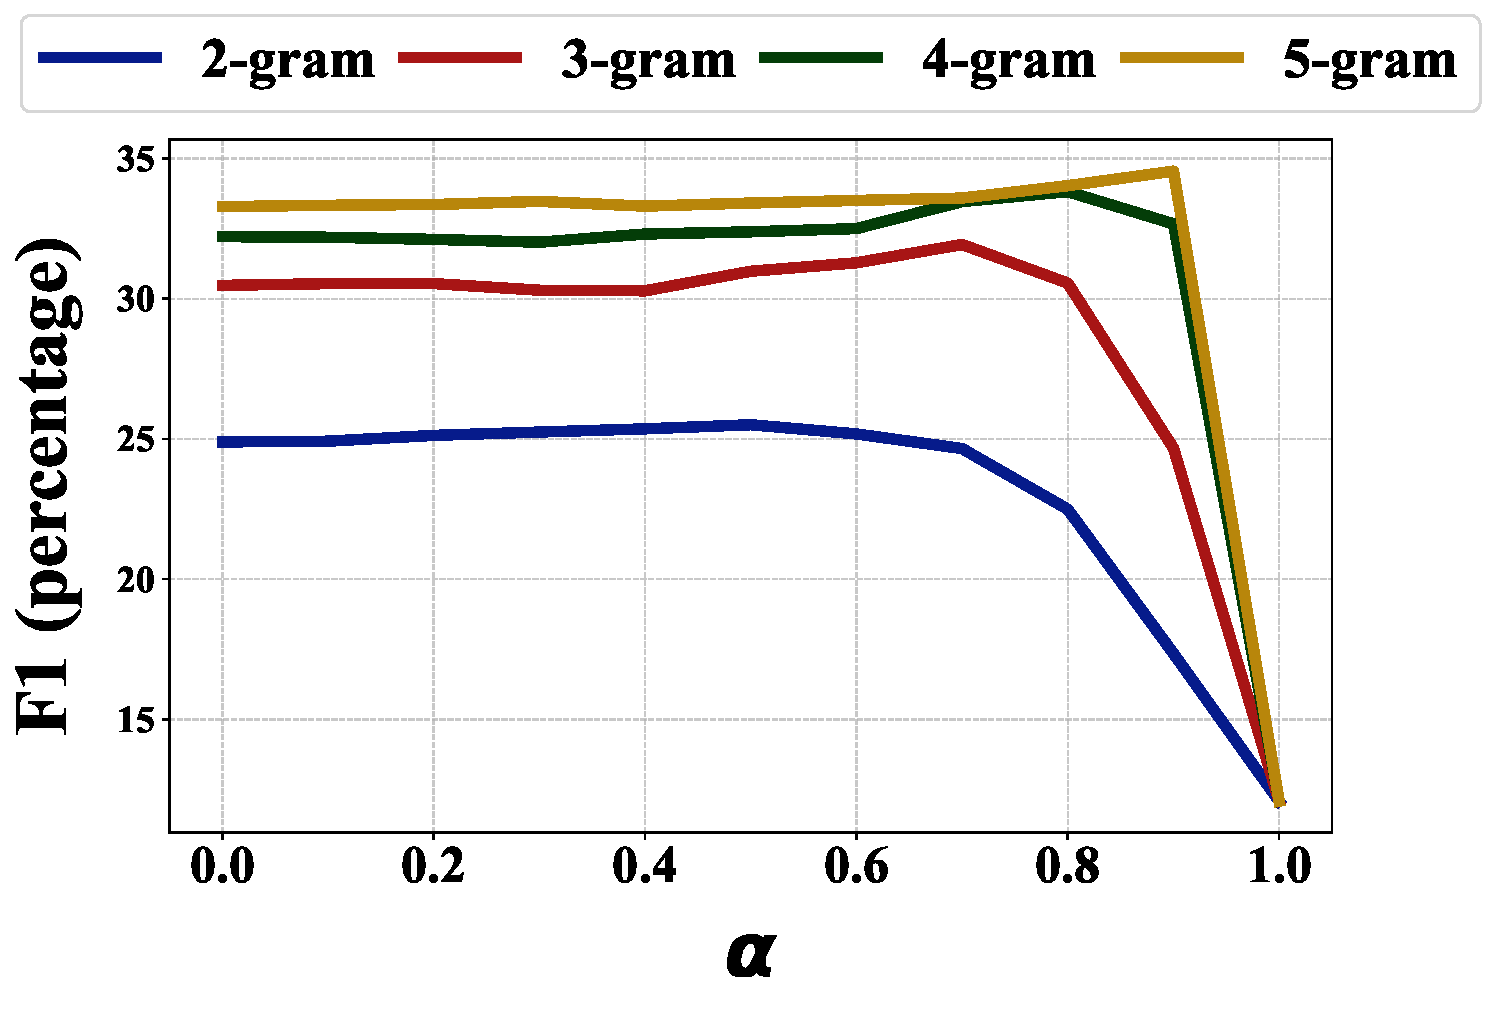
\includegraphics[width=\linewidth]{./images/ensemble-event-prec.pdf}
  \caption{PCR on Event-GNN + BM25}
  \label{fig:ensemble/eventprec}
\end{subfigure}%
\begin{subfigure}[t]{.32\textwidth}
  \centering
  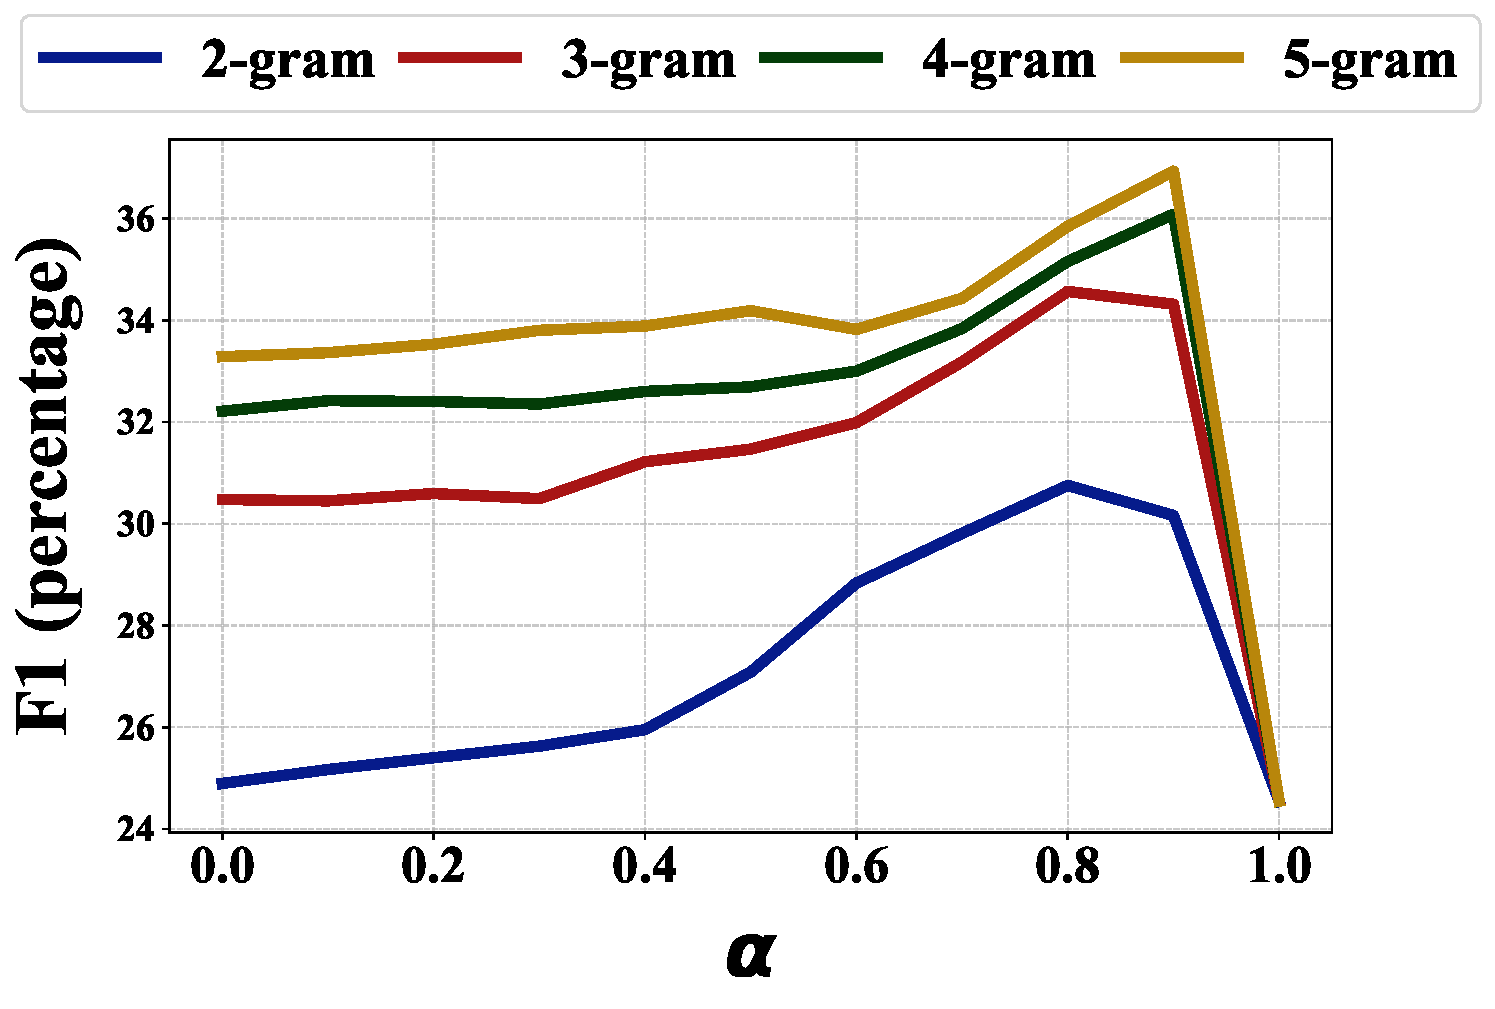
\includegraphics[width=\linewidth]{./images/ensemble-para-prec.pdf}
  \caption{PCR on Para-GNN + BM25}
  \label{fig:ensemble/paraprec}
\end{subfigure}%
\begin{subfigure}[t]{.32\textwidth}
  \centering
  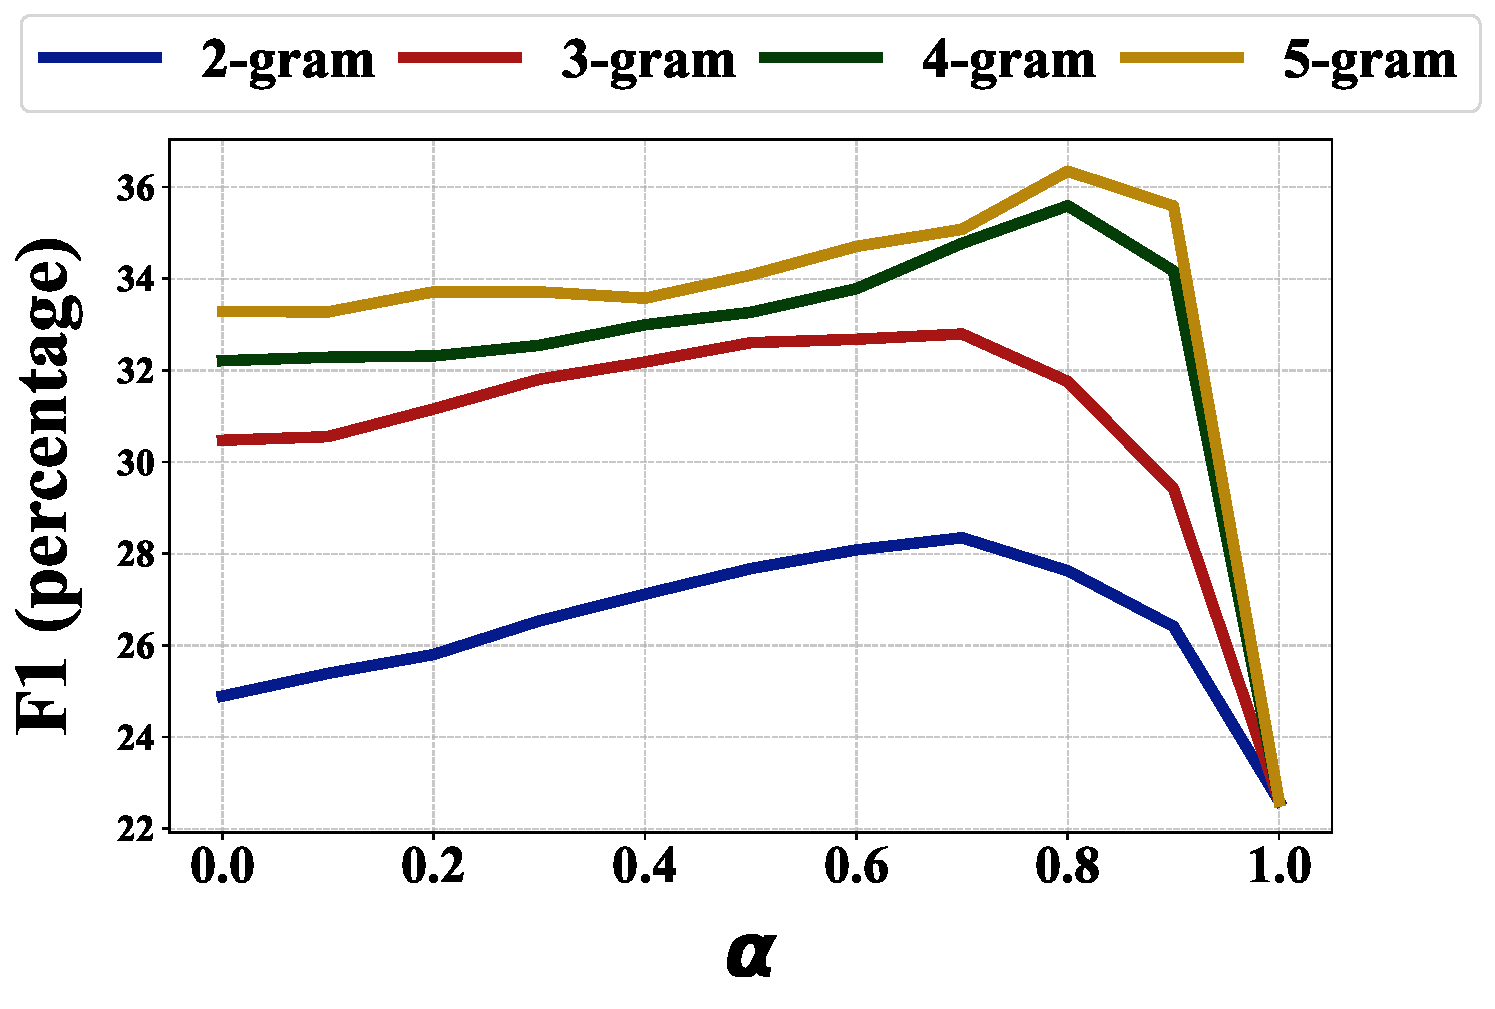
\includegraphics[width=\linewidth]{./images/ensemble-summ-prec.pdf}
  \caption{PCR on Para-GNN (summaries) + BM25}
  \label{fig:ensemble/summprec}
\end{subfigure}%
%\vspace{-4mm}
\caption{Grid Search F1(\%) of the ensemble methods for PCR task. Each figure shows the plot of performance vs. different $\alpha$ values when combining different models with BM25.} 
\label{fig:ensemble-precalpha}
%\vspace{-5mm}
\end{figure*}

\vspace{1mm}
\noindent \underline{\bf Dynamic $\alpha$ tuning:} Table~\ref{tab:dynalpha} compares the observations from grid search with the dynamic $\alpha$ method. For LSR, the learned weights (0.84–0.94) align closely with grid-search optima, confirming the \textit{semantic-heavy nature of statute retrieval}. For PCR, multi-task and transfer setups converge to values near the grid-search peaks (around 0.8), while independent fine-tuning collapses to a much lower $\alpha$ ($\sim$0.16), effectively over-weighting BM25. This explains why independent tuning lags behind, whereas transfer learning provides the most stable balance between semantic and lexical evidence. Overall, these findings reinforce the task asymmetry: \textit{LSR depends more on semantics, PCR more on lexical precision}, and ensembles are most effective when this balance is explicitly optimized.


\subsection{Statistical Significance Testing} \label{app:sigtest}
To confirm the reliability of our improvements, we performed paired $t$-tests on macro-F1 scores for the strongest ensemble and LLM-based models. We compared three ensemble variants of Para-GNN (summaries) + BM25 with dynamic $\alpha$ fine-tuning: (i)~fine-tuned separately (En-Sep), (ii)~fine-tuned in a multi-task setup (En-MT), and (iii)~fine-tuned with transfer learning (En-TL), along with the two prompting stages of GPT-4.1 re-ranking (GPT-S1 and GPT-S2). The resulting $p$-values are reported in Table~\ref{tab:sigtest}.

\begin{table}[!ht]
    \centering
    \small
    \begin{tabular}{llcc}
        \toprule
         \textbf{Method 1} & \textbf{Method 2} & \textbf{LSR $p$-val} & \textbf{PCR $p$-val} \\ 
         \midrule
         En-Sep & En-MT  & 6.8e-4  & 5e-1 \\
         En-Sep & En-TL  & 4.3e-4  & 8e-2 \\
         En-MT  & En-TL  & 8.4e-8  & 9.1e-3 \\
         En-Sep & GPT-S1 & 4.6e-32 & 6.1e-7 \\
         En-MT  & GPT-S1 & 5.3e-34 & 1.2e-10 \\
         En-TL  & GPT-S1 & 1.5e-29 & 2.2e-8 \\
         GPT-S1 & GPT-S2 & 1.8e-3  & 3.2e-3 \\
         \bottomrule
    \end{tabular}
    \caption{$p$-values from paired $t$-tests over macro-F1 scores for LSR and PCR among top-performing models.}
    \label{tab:sigtest}
\end{table}

\noindent Within the ensemble family, transfer learning (En-TL) consistently yields significant gains over both separate and multi-task fine-tuning, reinforcing its effectiveness for leveraging cross-task knowledge. More importantly, GPT-S1 significantly outperforms all ensemble variants by large margins ($p \ll 0.01$), establishing LLM re-ranking as clearly superior to traditional ensembles. Finally, the improvements of GPT-S2 over GPT-S1 are themselves statistically significant for both LSR and PCR, underscoring the benefit of incorporating cross-task dependencies in the second-stage prompt.


\begin{table*}
    \centering
    \begin{tabular}{|p{0.99\textwidth}|}
    \hline
    You are a smart and diligent Indian legal assistant with expertise in analyzing court judgments and identifying cited statutory provisions.

Context:

You will be provided with: \\
- A masked judgment: All statute names and section numbers have been replaced with placeholders like [ACT], [SECTION], etc.
- A **list of statutory sections**: Each entry includes a unique ID, and the name of the corresponding statute.

**Your Task:**

1. **Analyze the Masked Judgment:**
   - Carefully interpret the masked judgment's legal reasoning and context.

2. **Understand the Statutory List:**
   - Review the provided statute list. 

3. **Determine Cited Statutes:**
   - Identify the statute sections that are cited  in the judgment.
   - Return only the relevant **IDs** of the cited statute sections.\\
    \hline
    \end{tabular}
    \caption{Prompt used for LLM Re-ranking Statutes }
    \label{tab:qry-stat-rerank}
\end{table*}

\begin{table*}
    \centering
    \begin{tabular}{|p{0.99\textwidth}|}
    \hline
    You are a indian legal AI assistant.

Your task is to decide whether the given precedent judgment is cited by the masked query judgment. The query text may include masked placeholders like [PRECEDENT], [ACT], or [SECTION].

Return YES if the query judgment cites the precedent judgment, otherwise return NO. 

Output Format:
'Respond with exactly one word: "YES" or "NO". '
'Do not include any explanation, punctuation, or additional text.'\\
    \hline
    \end{tabular}
    \caption{Prompt used for LLM Re-ranking Precedents Stage 1 }
    \label{tab:qry-prec-rerank1}
\end{table*}

\begin{table*}
    \centering
    \begin{tabular}{|p{0.99\textwidth}|}
    \hline
    You are a indian legal AI assistant.

Your task is to decide whether the given precedent judgment is cited by the masked query judgment. The query text may include masked placeholders like [PRECEDENT], [ACT], or [SECTION]. To assist your decision, statute cited in both the query and precedent are provided.

Return YES if the query judgment cites the precedent judgment, otherwise return NO. 

Output Format:
'Respond with exactly one word: "YES" or "NO". '
'Do not include any explanation, punctuation, or additional text.'\\
    \hline
    \end{tabular}
    \caption{Prompt used for LLM Re-ranking Precedents Stage 2 }
    \label{tab:qry-prec-rerank2}
\end{table*}



% \begin{figure*}
% \begin{subfigure}[t]{.48\textwidth}
%   \centering
%   \includegraphics[width=\linewidth]{./images/freq_analysis_stats.png}
%   \caption{LSR}
%   \label{fig:freq-analysis-lsr}
% \end{subfigure}%
% \begin{subfigure}[t]{.48\textwidth}
%   \centering
%   \includegraphics[width=\linewidth]{./images/freq_analysis_precs.png}
%   \caption{PCR}
%   \label{fig:freq-analysis-pcr}
% \end{subfigure}%
% \caption{Performance in terms of F1(\%) compared to frequency of candidates. On the X-axis, the candidates are sorted from left to right according to frequency and divided into groups (most frequent group 1, most rare group 5). We compare the Ensemble model (Para-GNN + BM25) under two settings, using full documents vs. summaries. Figure~\ref{fig:freq-analysis-lsr} shows LSR performance and Figure~\ref{fig:freq-analysis-pcr} shows PCR performance.} 
% \label{fig:freq-analysis}
% %\vspace{-5mm}
% \end{figure*}

\begin{figure*}
\begin{subfigure}[t]{.5\linewidth}
  \centering
  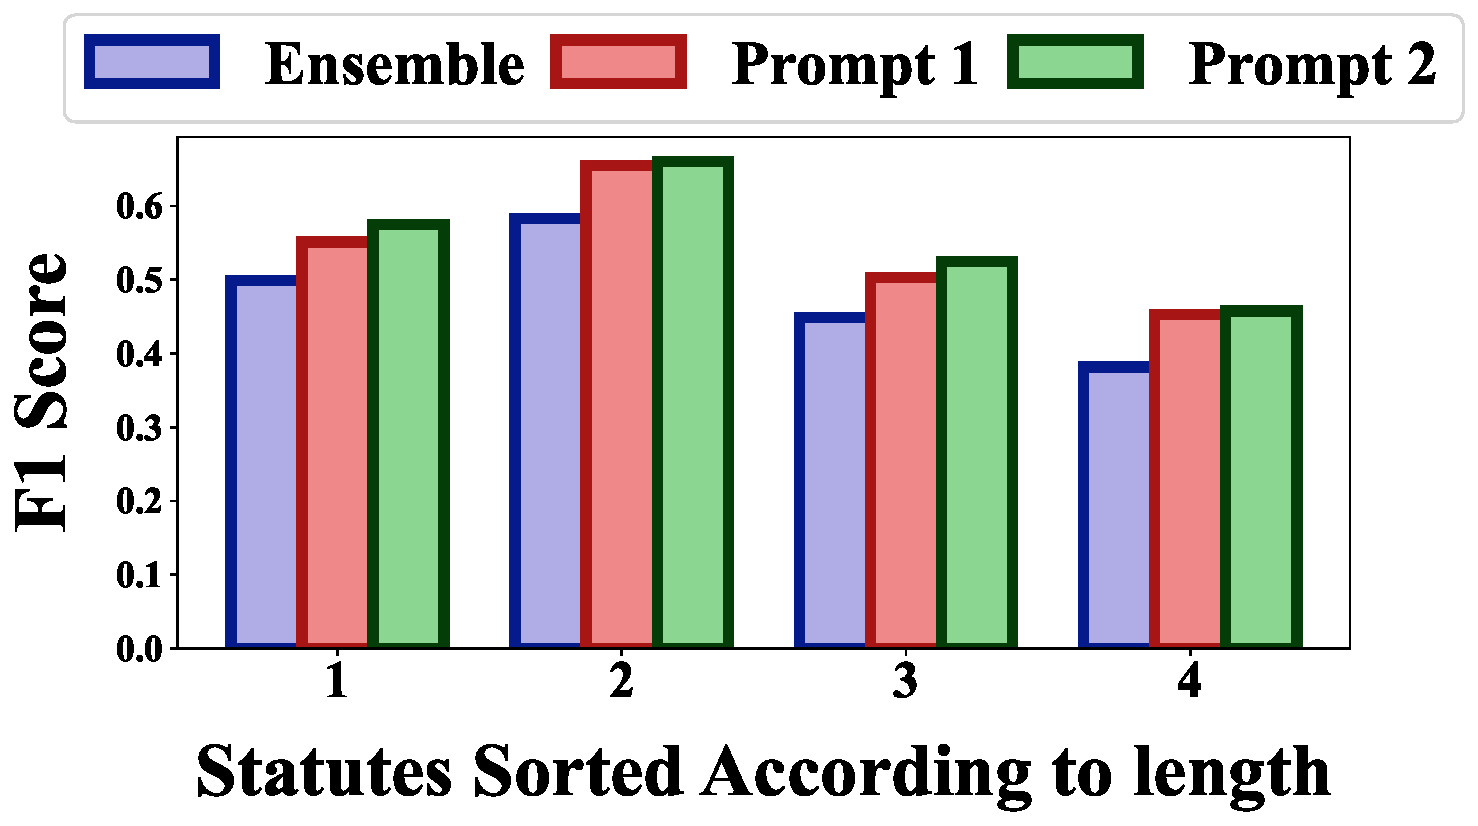
\includegraphics[width=\linewidth]{./images/llm-len-stats.pdf}
  \caption{LSR F1 vs. stat length}
  \label{fig:llm-len-stats}
\end{subfigure}%
\begin{subfigure}[t]{.5\linewidth}
  \centering
  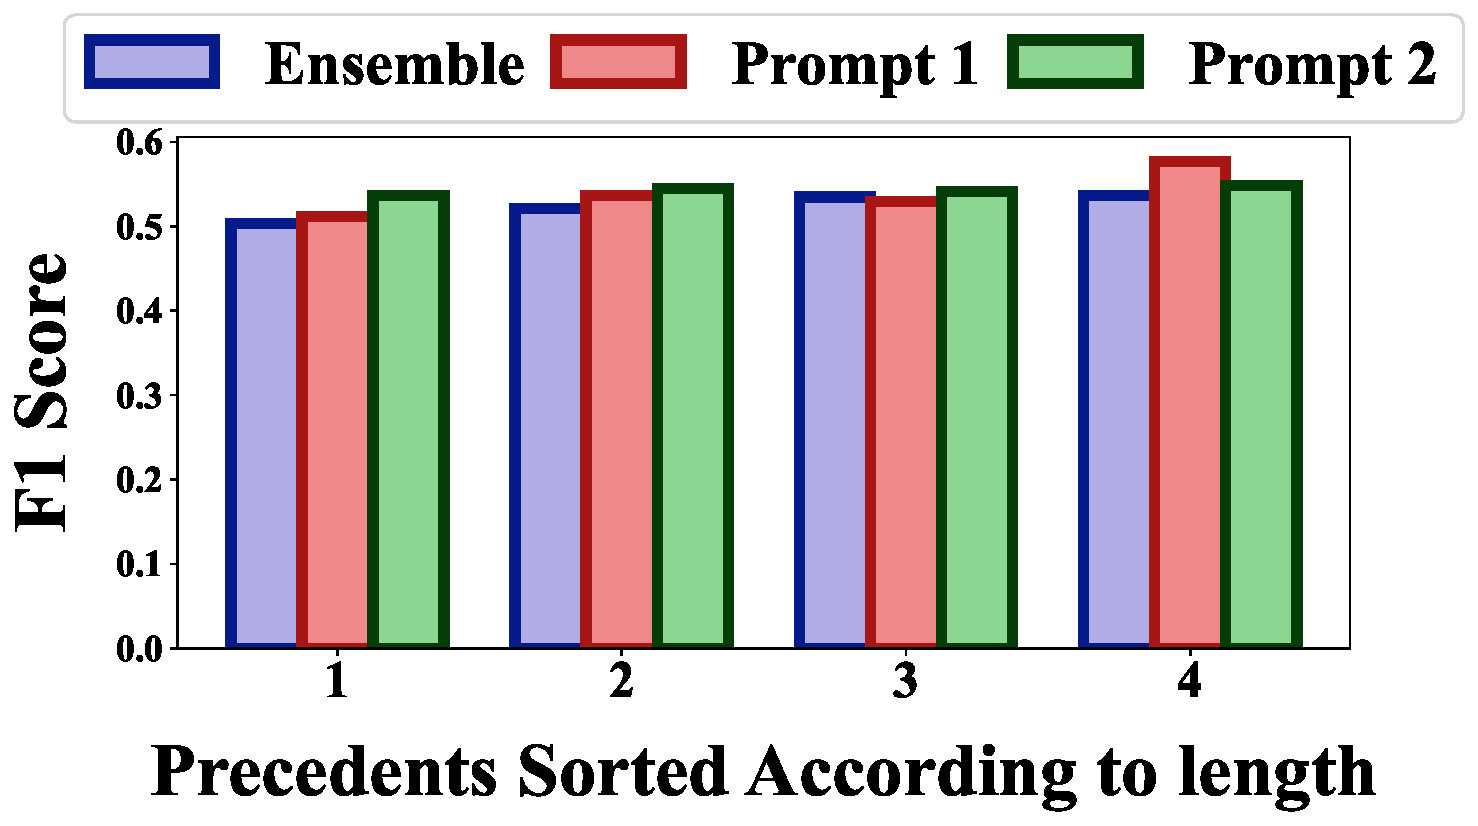
\includegraphics[width=\linewidth]{./images/llm-len-precs.pdf}
  \caption{PCR F1 vs. prec length}
  \label{fig:llm-len-precs}
\end{subfigure}%
\vspace{-2mm}
\caption{Performance in terms of F1(\%) compared to \textit{candidate} text lengths. On the X-axis, the candidates are sorted from left to right according to text length and divided into groups (shortest candidates group 1, longest candidates group 4). Figure~\ref{fig:llm-len-stats} shows LSR performance and Figure~\ref{fig:llm-len-precs} shows PCR performance with varying candidate (statute and precedent respectively) lengths.} 
\label{fig:llm-len-cands}
% \vspace{-5mm}
\end{figure*}



\begin{figure*}
\begin{subfigure}[t]{.5\linewidth}
  \centering
  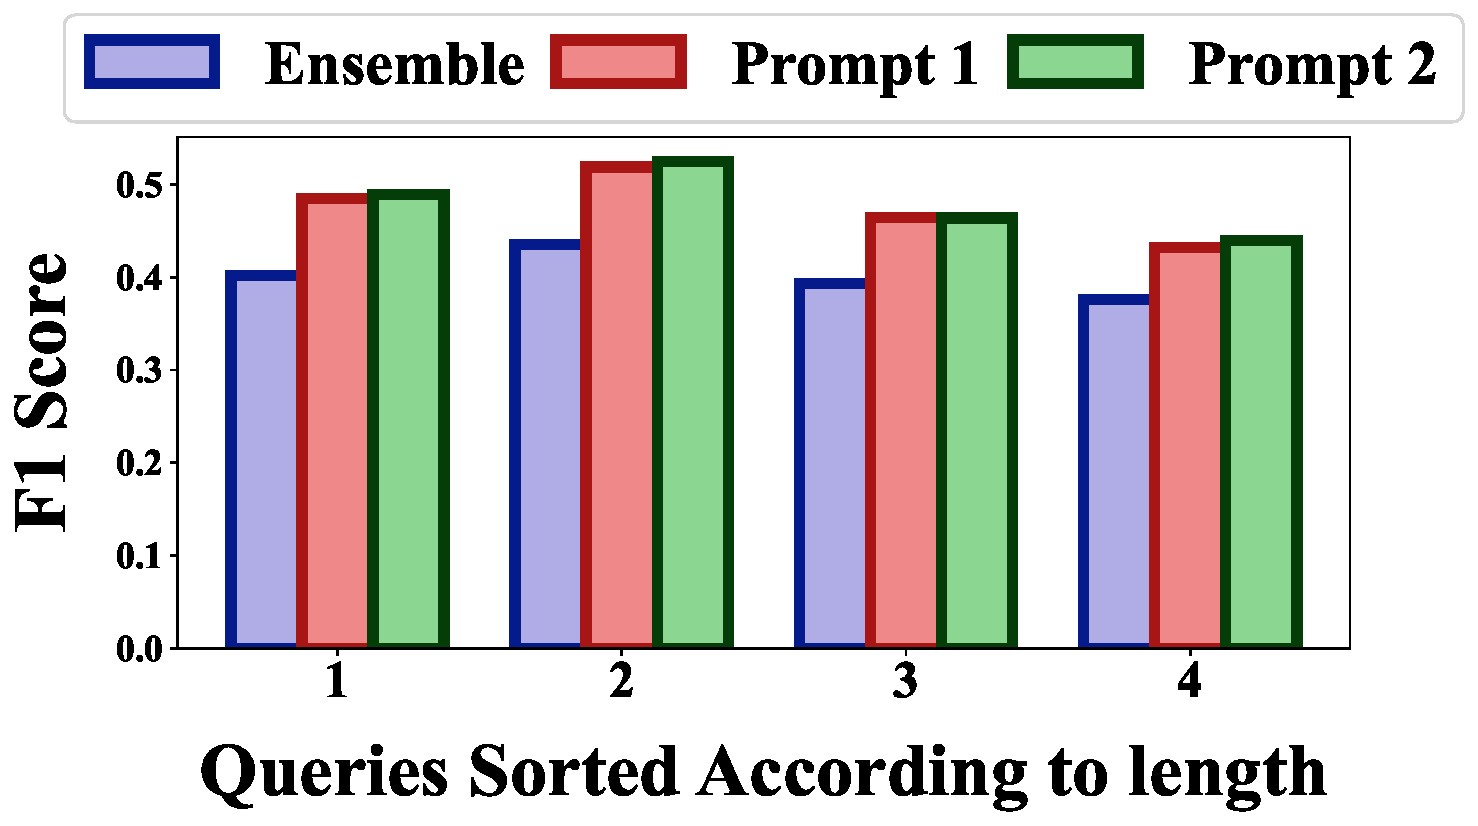
\includegraphics[width=\linewidth]{./images/llm-len-qry-lsr.pdf}
  \caption{LSR F1 vs. query length}
  \label{fig:llm-len-qry-lsr}
\end{subfigure}%
\begin{subfigure}[t]{.5\linewidth}
  \centering
  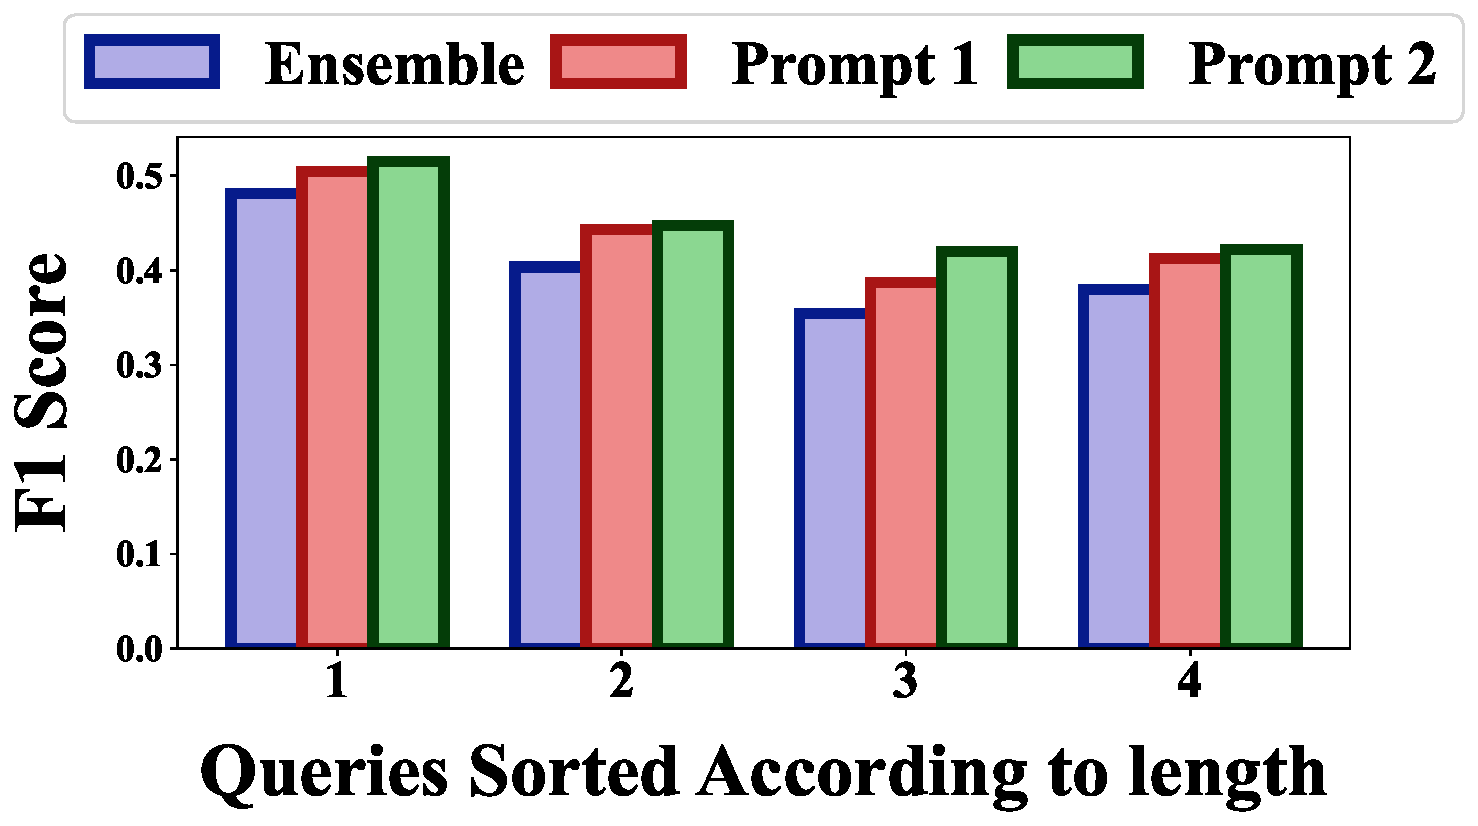
\includegraphics[width=\linewidth]{./images/llm-len-qry-pcr.pdf}
  \caption{PCR F1 vs. query length}
  \label{fig:llm-len-qry-pcr}
\end{subfigure}%
\vspace{-2mm}
\caption{Performance in terms of F1(\%) compared to \textit{query} text lengths. On the X-axis, the queries are sorted from left to right according to text length and divided into groups (shortest candidates group 1, longest candidates group 4). Figure~\ref{fig:llm-len-stats} shows LSR performance and Figure~\ref{fig:llm-len-precs} shows PCR performance with varying query lengths.} 
\label{fig:llm-len-qry}
% \vspace{-5mm}
\end{figure*}

\subsection{Analyzing the effect of candidate frequencies and text lengths} \label{app:freqlenanalysis}

% \paul{As discussed in Section~\ref{sec:expt}, the first stage LLM prompting improves upon the ensemble-based retriever across all ranges of candidate frequencies for both LSR and PCR, while the second-stage prompting mostly improves over the relatively frequent statutes (see Figure~\ref{fig:llm-freq}).}


% We also observe for all models, the fine-tuned model is able to achieve a performance close to the grid-search approach (see Table~\ref{tab:results}), which suggests that there is enough signal in the data to learn the optimal $\alpha$ ratio. On inspecting the average $\alpha$ values generated over the test set, we notice that $\alpha=0.94$ for statutes and $\alpha=0.78$ for precedents in the case of Event-GNN. For Para-GNN, the average values are $\alpha=0.85$ and $\alpha=0.82$ for statutes and precedents respectively. In case of Para-GNN with summaries, the average values are $\alpha=0.95$ and $\alpha=0.80$ for statutes and precedents respectively. Nevertheless, the ensemble models outperform the individual lexical and semantic approaches. 
We analyzed how the performance of the best models vary across candidates of different frequency ranges in \S~\ref{sec:expt} (Fig.~\ref{fig:llm-freq}). We conduct a more in-depth analysis of the effect of candidate frequency, as well as length of query and candidate texts in this Section.

\vspace{1mm}
\noindent\underline{\bf Held-out and Never-cited Candidates:} \label{app:heldout}
To analyze robustness, we study two challenging candidate types:  
(i)~\textit{held-out candidates}, i.e., statutes/precedents cited only in the test set but absent from train/dev, and  
(ii)~\textit{never-cited candidates}, i.e., candidates that are never cited in any query. 
\ilpcsr{} consists of 20 held-out statutes and 88 precedents. There are 19 never-cited statutes and 93 such precedents (Table~\ref{tab:salient-stats-ilpcsr}, App.~\ref{sec:dataset-appendix}).

\noindent {\bf Held-out candidates:} We restrict evaluation to queries that cite at least one such candidate, and compute F1 over this restricted set. Results are shown in Table~\ref{tab:heldout} (same notations for models as the above Section). For LSR, En-MT achieves the best generalization, while En-Sep lags behind. For PCR, En-Sep performs best, but differences across ensembles and GPT re-ranking are relatively small. Importantly, GPT-based re-ranking does not provide additional gains here, suggesting that ensembles remain highly competitive when generalizing to unseen candidates.

\begin{table}[!ht]
\centering
\small
\begin{tabular}{lcc}
\toprule
\textbf{Model} & \textbf{LSR F1} & \textbf{PCR F1} \\
\midrule
En-Sep  & 33.33 & 64.29 \\
En-MT   & \textbf{40.00} & 58.39 \\
En-TL   & 38.67 & 58.04 \\
GPT-S1  & 38.67 & 58.04 \\
GPT-S2  & 38.67 & 58.04 \\
\bottomrule
\end{tabular}
\caption{Performance (macro-F1, percentage) on held-out candidates.}
\label{tab:heldout}
\end{table}

\noindent {\bf Never-cited candidates:} We count the number of test queries where at least one never-cited candidate is ranked in the top-5 (Table~\ref{tab:nevercited}). A higher value indicates poorer robustness, since irrelevant candidates should not be prioritized. Here, we find that LSR is largely unaffected (almost no spurious never-cited retrievals), while PCR is more sensitive. Among ensembles, En-Sep shows the worst robustness, while En-MT and En-TL reduce false retrievals. GPT re-ranking performs comparably to the stronger ensembles, indicating that while LLMs offer gains on cited candidates, they do not exacerbate errors from never-cited ones.

\begin{table}[!ht]
\centering
\small
\begin{tabular}{lcc}
\toprule
\textbf{Model} & \textbf{LSR} & \textbf{PCR} \\
\midrule
En-Sep  & 0 & 35 \\
En-MT   & 3 & 23 \\
En-TL   & 0 & 26 \\
GPT-S1  & 1 & 24 \\
GPT-S2  & 1 & 24 \\
\bottomrule
\end{tabular}
\caption{Number of test queries where a never-cited candidate appears in top-5. Lower is better.}
\label{tab:nevercited}
\end{table}

\noindent Overall, these analyses show that while GPT-based re-ranking provides state-of-the-art gains on cited candidates, ensembles retain strong robustness on both held-out and never-cited cases. LSR models are inherently more resistant to never-cited noise, whereas PCR models require better mechanisms to handle such distractors.


%%%%%%%%%%%%%%%%%%%%%%%%%%%%%%%%%%%%%%%%%%%%%%%%%%%



% Both statutes and precedents are not uniformly distributed in the dataset, usually both these follow a long tail distribution (some candidates are cited by most queries, most other candidates are cited by few). Thus, it is interesting to analyze the performance of different models on different candidates based on their frequency of citation.
% Figure:~\ref{fig:freq-analysis} shows the performance of the Para-GNN + BM25 Ensemble (Grid Search) model with two variations, using full documents vs. summaries as input. We divide the candidate spaces into 5 equal-sized, disjoint groups based on frequency, and plot the F1 scores for each group considering only those candidates in the given group. On the query side, we only include those queries for evaluation that cite at least one candidate in the group. Naturally, groups containing frequently cited candidates are larger in size than the ones containing rare candidates.

% We observe that for statutes, the frequency plays a very crucial role, with the performance decreasing sharply across the most rare groups (Groups 4-5). The difference in performance of the model, when using summaries compared to full documents, is larger for the frequent groups, which got tuned better with the summaries. For precedents, frequency seems to play a much lesser role, with the performance on the rare groups being similar to the frequent groups. It is also interesting to note that there is a significant drop in performance for the summary-based model over Group-5 (most rare precedents). Thus, for both LSR and PCR, the summary-based methods lose their efficacy over the rare candidates.

% \noindent\textbf{Performance over held-out Candidates:}
% % As discussed in Section~\ref{sec:dataset/overview}, the \ilpcsr{} dataset contains some candidates that are not cited by any training queries but stil cited by some test queries, which can be considered as held-out candidates. There are 29 such statutes and 155 such precedents.
% \paul{[TO WRITE]}


% \begin{table}
%     \centering
%     \small
%     \setlength{\tabcolsep}{3pt}
%     \begin{tabular}{p{0.25\textwidth}cc}
%         \hline
%         \textbf{Method} & \textbf{Statutes} & \textbf{Precedents} \\ \hline
%          Event-GNN + BM25 & \textbf{37.03} & 42.88 \\
%          Para-GNN + BM25 & 28.70  & 53.18 \\
%          Para-GNN (summaries) + BM25 & \textbf{37.03}  & \textbf{54.30} \\ \hline
%     \end{tabular}
%     \caption{Performance in macro-F1@$K$ (\%) for the best ensemble methods on the zero shot candidates for \ilpcsr{}}
%     \label{tab:held-out}
% \end{table}

% Table~\ref{tab:held-out} shows the performance of the best-performing ensemble methods for the zero shot candidates. The trends for the held-out candidates follow those for the entire candidate space -- Event-GNN and Para-GNN (summaries) perform best for LSR, whereas Para-GNN (full doc) and Para-GNN (summaries) perform well for PCR. Overall, for both tasks, Para-GNN (summaries) perform the best for the held-out candidates.



%%%%%%%%%%%%%%%%%%%%%%%%%%%%%%%%%%%%
\noindent\underline{\bf Analyzing the effect of text lengths:} \label{app:lenanalysis}
% \section{Analysis with Text Lengths} \label{app:lenanalysis}
We also analyze the effect of text lengths on retrieval performance, considering both queries and candidates. For each case, we sort the documents by their token length and divide them into four groups (Group-1 containing the shortest, Group-4 containing the longest). The grouping procedure is consistent with the frequency-based analysis in \S~\ref{sec:expt}, ensuring comparability across different perspectives of candidate/query difficulty. We then evaluate performance using the same set of methods considered in \S~\ref{sec:expt}, and report macro-F1 scores. Results are shown in Fig.~\ref{fig:llm-len-cands} for candidates and Fig.~\ref{fig:llm-len-qry} for queries.  

\noindent\textbf{Varying Candidate Lengths:}  
As shown in Fig.~\ref{fig:llm-len-cands}, LLM re-ranking consistently outperforms ensembles across candidate length groups. For LSR, Stage-2 prompting provides the largest benefits for shorter and medium-length statutes, while for PCR the improvements are strongest on longer precedents, where the LLM’s ability to capture nuanced reasoning helps counteract noise in extended case texts.  

\noindent\textbf{Varying Query Lengths:}  
From Fig.~\ref{fig:llm-len-qry}, we observe that LLMs achieve substantial gains on short queries in both LSR and PCR, suggesting that they are able to compensate for missing details through contextual reasoning. While the gains on longer queries are smaller, they remain steady, ensuring that LLMs maintain superiority over ensemble methods across all groups.  

\noindent Candidate length mainly affects how models handle verbosity, with LLMs showing clear benefits on long precedents and short statutes. Query length highlights the ability of LLMs to recover missing context, especially for shorter queries. Overall, LLM re-ranking remains robust across both query and candidate length variations.

\section{Details of the Annotation Study} \label{app:annot}

As described in \S~\ref{sec:human-annotation}, we conducted an annotation study with domain experts to examine the subjectivity of legal relevance. Six senior LL.M. students (aged 24–28) carried out the annotations under the supervision of a senior faculty member, all from the WB National University of Juridical Sciences. All annotators were informed of the study’s purpose and provided explicit consent for the use of their data. The annotators (Law students) agreed to perform the annotations on pro-bono basis as they were curious about AI technology and how it can be improved for the Law domain. To further mitigate potential biases, we manually ensured that all 60 query documents were completely anonymized prior to annotation, ensuring that no demographic or sensitive information could influence the process.




%\vspace{-2mm}
\section{Experiments on COLIEE dataset} \label{sec:coliee}
%\vspace{-3mm}

\begin{table}[t]
    \centering
    %\small
    \small
    \setlength{\tabcolsep}{5pt}
    \begin{tabular}{p{0.1\textwidth}cccc}
        \toprule
        \textbf{Model} &  \multicolumn{2}{c}{\textbf{Statutes}}&  \multicolumn{2}{c}{\textbf{Precedents}}\\
         &  \ilpcsr &  \coliee &  \ilpcsr &  \coliee \\ \midrule
         BM25 (5-gram)&  16.98&  54.49&  33.29& 30.61\\
         Event-GNN&  28.67& - &  12.08& 11.48 \\
         Para-GNN&  20.72&  17.64&  24.54& 21.24\\
 Para-GNN (summaries)& & -& &18.52\\ \midrule
         Para-GNN + BM25&  28.10 & 55.96&  \textbf{36.93} & \textbf{34.52}\\
Event-GNN + BM25& 33.87& -& 34.45&34.51\\ 
 Para-GNN (summaries) + BM25& \textbf{36.17} & -& 36.35&30.25\\ \bottomrule
    \end{tabular}
    \vspace{-3mm}
    \caption{Results of the best methods on \coliee{} datasets compared to ILPCSR. All results are in terms of macro-F1@$K$. Event-GNN and summaries could not be run for \coliee{} statutes since the queries are too small for meaningful events or summaries.}
    \label{tab:coliee}
    \vspace{-6mm}
\end{table}

All our observations are drawn over the \ilpcsr{} dataset constructed in this work. We would like to verify whether the above trends are also seen on other legal datasets/jurisdictions. Since no current dataset allows the identification of both statutes and precedents together from the same query, we have to work with two separate datasets for LSR and PCR. We choose to work on the well-known COLIEE datasets~\cite{li2024coliee2024}. 
%Specifically, we use the COLIEE 2024 Task 1 (Legal Precedent Retrieval) and Task 3 (Statute Law Retrieval) datasets for the tasks of LSR and PCR respectively. 

\noindent\underline{\textbf{LSR dataset:}} We use the \texttt{COLIEE 2024 Task 3 (Statute Law Retrieval)} dataset consisting of 746 statutes from \textit{Japanese law}, and 554 queries. Note that the queries here are typically one or two sentences long, asking specifically about the laws. 
In contrast, the queries in \ilpcsr{} are real-life cases, which makes the setting more practical and challenging. 
We opted for this dataset since other existing datasets in English (ECHR2021 and ILSI) have too less statutes  (66 and 100 respectively) to be evaluated in the retrieval setup. 

\noindent \underline{\textbf{PCR dataset:}} We use the \texttt{COLIEE 2024 Task 1 (Legal Precedent Retrieval)} dataset consisting of 1,678 queries and 5,529 precedent candidates, all of which are real-life case judgments from \textit{Canadian Federal law}. This setting is similar to the queries in \ilpcsr{}. 

\noindent \underline{\textbf{Results:}}
We choose some of the methods that performed highly over the \ilpcsr{} dataset, and applied these methods on the COLIEE datasets.
The results on \coliee{} vis-a-vis \ilpcsr{} are presented in Table~\ref{tab:coliee}.
The trends on the \coliee{} dataset are almost similar to what we observed for \ilpcsr{}. 
The only difference being that, for \coliee{}, even for LSR, lexical methods such as BM25 perform the best (whereas semantic methods outperformed lexical approaches for LSR in \ilpcsr{}). 
This difference is possibly because the queries of \coliee{} are short sentences, asking directly about the statutes, whereas for \ilpcsr{} the queries are real-world long case judgments. Both for LSR and PCR, we see improvements when using an ensemble setup for \coliee{} as well. The improvement is limited in case of statutes, possibly because the performance of Para-GNN is poor. This is possibly because short queries do not have enough structure for the GNN to exploit. For precedents, where the semantic methods perform better, the improvement obtained by ensembling is high. 
This agrees with the trend we see on \ilpcsr{} (see Table~\ref{tab:coliee}). Finally, for both \ilpcsr{} and \coliee{}, in the case of PCR, we have observed that using summaries does not perform as well as using the full texts. We observe the same key findings as \ilpcsr. 
